\chapter{Funciones vectoriales y funciones de varias variables}
\label{ch:vector-multivariable}

Las funciones que asocian a un número real un vector en el plano o en el
espacio —las \textbf{funciones vectoriales}— constituyen el lenguaje
natural para describir trayectorias de partículas, curvas en el espacio
y campos de fuerzas. Su estudio requiere extender al ámbito vectorial
los conceptos centrales del cálculo diferencial e integral: límite,
continuidad, derivada e integral. Esta extensión resulta
sorprendentemente directa: cada operación se aplica \emph{componente a
componente}, de modo que el cálculo con funciones vectoriales hereda las
reglas del cálculo escalar sin necesidad de desarrollar una teoría
completamente nueva.

A continuación, las funciones que dependen de \emph{dos o más variables
independientes} —las \textbf{funciones de varias variables}— abren la
puerta al cálculo multivariable propiamente dicho. Aquí el dominio deja
de ser un subconjunto de la recta real para convertirse en una región
del plano o del espacio; la gráfica, cuando existe, es una superficie en
$\mathbb{R}^3$; y la visualización de los valores constantes de la
función se logra mediante curvas y superficies de nivel. Estos
conceptos, aparentemente geométricos, son la base sobre la que se
construirán más adelante las derivadas parciales, las integrales
múltiples y el cálculo vectorial.

\section{Funciones vectoriales}
\label{sec:vector-functions}
\begin{definition}[Función vectorial]
Una \textbf{función vectorial} es una regla que asigna a cada número
real $t$ de su dominio un único vector $\mathbf{r}(t)$ en
$\mathbb{R}^2$ o en $\mathbb{R}^3$. Mientras que una función escalar
produce un número real como salida, una función vectorial produce una
cantidad con dirección y magnitud.

Si una partícula se mueve en el espacio y en cada instante $t$ ocupa una
posición determinada, su movimiento se describe mediante una función
vectorial
\[
\mathbf{r}(t) = \langle f(t), g(t), h(t) \rangle,
\]
donde $f$, $g$ y $h$ son funciones reales llamadas \textbf{componentes}
de $\mathbf{r}$. Cada componente indica cómo varía la posición en una
de las direcciones coordenadas: $x$, $y$ y $z$, respectivamente.

En el plano, la notación se reduce a
\[
\mathbf{r}(t) = f(t)\,\mathbf{i} + g(t)\,\mathbf{j},
\]
y en el espacio tridimensional,
\[
\mathbf{r}(t) = f(t)\,\mathbf{i} + g(t)\,\mathbf{j} + h(t)\,\mathbf{k}.
\]
\end{definition}
El dominio de $\mathbf{r}$ es la intersección de los dominios de sus
funciones componentes; es decir, $t$ debe pertenecer al dominio de
$f$, de $g$ y de $h$ simultáneamente. La imagen de $\mathbf{r}$ es una
curva en $\mathbb{R}^2$ o $\mathbb{R}^3$, denominada \textbf{trayectoria}
o \textbf{curva parametrizada}.

\begin{figure}[H]
\centering
\begin{tikzpicture}
\begin{axis}[
    view={35}{20},
    xlabel={$x$}, ylabel={$y$}, zlabel={$z$},
    axis lines=center,
    tick style={thin},
    xtick={-1,0,1}, ytick={-1,0,1}, ztick={0,1,2,3},
    width=8cm, height=8cm,
]
    \addplot3[
        thick, blue!70!black,
        domain=0:6.2832,
        samples=50,
        samples y=0,
    ] ({cos(deg(x))}, {sin(deg(x))}, {x/2});
    \addplot3[only marks, mark=*, mark size=2pt, red!70!black]
        coordinates {(0,1,0.785)};
    \draw[->, thick, red!70!black]
        (axis cs:0,1,0.785) -- (axis cs:-0.4,1,0.985);
    \node[above left] at (axis cs:-0.4,1,0.985)
        {\small $\mathbf{r}'(\tfrac{\pi}{2})$};
\end{axis}
\end{tikzpicture}
\caption{Hélice $\mathbf{r}(t)=(\cos t,\sin t,\tfrac{t}{2})$,
         $t\in[0,2\pi]$, con vector tangente en $t=\tfrac{\pi}{2}$}
\label{fig:helice_tangente}
\end{figure}

\subsection{Límite de una función vectorial}

El límite de una función vectorial describe el comportamiento del vector
$\mathbf{r}(t)$ cuando el parámetro $t$ se aproxima a un valor $a$.
Intuitivamente, $\mathbf{r}(t)$ se acerca a un vector $\mathbf{u}$
si, a medida que $t$ tiende a $a$, cada componente de $\mathbf{r}(t)$
se aproxima a la componente correspondiente de $\mathbf{u}$.

\begin{definition}[Límite de una función vectorial]
Sea $\mathbf{r}(t) = \langle f(t), g(t), h(t) \rangle$ definida en un
entorno de $a$ (excepto, posiblemente, en $a$ mismo). Se dice que el
límite de $\mathbf{r}(t)$ cuando $t$ tiende a $a$ es el vector
$\mathbf{u} = \langle u_1, u_2, u_3 \rangle$, y se escribe
\[
\lim_{t \to a} \mathbf{r}(t) = \mathbf{u},
\]
si y solo si
\[
\lim_{t \to a} f(t) = u_1, \qquad
\lim_{t \to a} g(t) = u_2, \qquad
\lim_{t \to a} h(t) = u_3.
\]
Equivalentemente,
\[
\lim_{t \to a} \mathbf{r}(t)
= \left\langle \lim_{t \to a} f(t),\;
            \lim_{t \to a} g(t),\;
            \lim_{t \to a} h(t) \right\rangle.
\]
\end{definition}

\begin{rem}
El límite de una función vectorial existe si y solo si existen los
límites de \emph{todas} sus componentes. Si alguna componente no tiene
límite en $a$, la función vectorial tampoco lo tiene. Esta propiedad
reduce el estudio de límites vectoriales al cálculo de límites escalares
familiares.
\end{rem}

\begin{example}[Cálculo de un límite vectorial]
Calcular
\[
\lim_{t \to 2} \left\langle t^2 - 1,\; \frac{t^2 - 4}{t - 2},\; \cos(\pi t) \right\rangle.
\]
\begin{myproof}
\textbf{Paso 1: Primera componente.}
\[
\lim_{t \to 2} (t^2 - 1) = 4 - 1 = 3.
\]

\textbf{Paso 2: Segunda componente.} Se simplifica antes de evaluar:
\[
\frac{t^2 - 4}{t - 2} = \frac{(t-2)(t+2)}{t-2} = t+2 \quad (t \neq 2),\quad
\lim_{t \to 2} \frac{t^2 - 4}{t - 2} = \lim_{t \to 2} (t+2) = 4.
\]

\textbf{Paso 3: Tercera componente.}
\[
\lim_{t \to 2} \cos(\pi t) = \cos(2\pi) = 1.
\]

\textbf{Paso 4: Resultado vectorial.}
\[
\boxed{\lim_{t \to 2} \left\langle t^2 - 1,\; \frac{t^2 - 4}{t - 2},\; \cos(\pi t) \right\rangle = \langle 3,\; 4,\; 1 \rangle}.
\]
\end{myproof}
\end{example}

\begin{prob}
Calcular el límite de cada función vectorial:
\begin{enumerate}[a)]
  \item $\displaystyle \lim_{t \to 0} \left\langle \frac{\sen t}{t},\; e^t,\; \frac{1-\cos t}{t} \right\rangle$.
  \item $\displaystyle \lim_{t \to 1} \left\langle t^2-1,\; \ln t,\; \frac{t^2-1}{t-1} \right\rangle$.
  \item $\displaystyle \lim_{t \to \infty} \left\langle \frac{t}{t+1},\; \frac{1}{t^2+1},\; \arctan t \right\rangle$.
\end{enumerate}
\begin{myproof}
El límite de una función vectorial se calcula componente a componente.

\textbf{Apartado a)} $\displaystyle\lim_{t\to 0}\!\left\langle\frac{\sen t}{t},\;e^t,\;\frac{1-\cos t}{t}\right\rangle$.

\textbf{Paso 1: Primera componente.} Límite trigonométrico fundamental:
\[
  \lim_{t\to 0}\frac{\sen t}{t} = 1.
\]

\textbf{Paso 2: Segunda componente.} $e^t$ es continua en $t=0$:
\[
  \lim_{t\to 0}e^t = e^0 = 1.
\]

\textbf{Paso 3: Tercera componente.} Forma $0/0$; se aplica L'Hôpital:
\[
  \lim_{t\to 0}\frac{1-\cos t}{t} = \lim_{t\to 0}\frac{\sen t}{1} = 0.
\]
\[
  \boxed{\lim_{t\to 0}\!\left\langle\frac{\sen t}{t},\;e^t,\;\frac{1-\cos t}{t}\right\rangle = \langle 1,\;1,\;0\rangle.}
\]

\textbf{Apartado b)} $\displaystyle\lim_{t\to 1}\!\left\langle t^2-1,\;\ln t,\;\frac{t^2-1}{t-1}\right\rangle$.

\textbf{Paso 1: Primeras dos componentes.} Son continuas en $t=1$:
\[
  \lim_{t\to 1}(t^2-1)=0,\qquad \lim_{t\to 1}\ln t = 0.
\]

\textbf{Paso 2: Tercera componente.} Forma $0/0$; se factoriza el numerador:
\[
  \lim_{t\to 1}\frac{t^2-1}{t-1}=\lim_{t\to 1}\frac{(t-1)(t+1)}{t-1}=\lim_{t\to 1}(t+1)=2.
\]
\[
  \boxed{\lim_{t\to 1}\!\left\langle t^2-1,\;\ln t,\;\frac{t^2-1}{t-1}\right\rangle = \langle 0,\;0,\;2\rangle.}
\]

\textbf{Apartado c)} $\displaystyle\lim_{t\to\infty}\!\left\langle\frac{t}{t+1},\;\frac{1}{t^2+1},\;\arctan t\right\rangle$.

\textbf{Paso 1: Primera componente.} Dividir por $t$:
\[
  \lim_{t\to\infty}\frac{t}{t+1}=\lim_{t\to\infty}\frac{1}{1+1/t}=1.
\]

\textbf{Paso 2: Segunda componente.} El denominador crece sin cota:
\[
  \lim_{t\to\infty}\frac{1}{t^2+1}=0.
\]

\textbf{Paso 3: Tercera componente.} Límite estándar de la arctangente:
\[
  \lim_{t\to\infty}\arctan t = \frac{\pi}{2}.
\]
\[
  \boxed{\lim_{t\to\infty}\!\left\langle\frac{t}{t+1},\;\frac{1}{t^2+1},\;\arctan t\right\rangle = \left\langle 1,\;0,\;\frac{\pi}{2}\right\rangle.}
\]
\end{myproof}
\end{prob}

\subsection{Continuidad de una función vectorial}

La continuidad de una función vectorial se define exigiendo que el
límite en un punto coincida con el valor de la función en ese punto, de
manera análoga al caso escalar.

\begin{definition}[Continuidad de una función vectorial]
Una función vectorial $\mathbf{r}(t) = \langle f(t), g(t), h(t) \rangle$
es \textbf{continua} en $t = a$ si
\[
\lim_{t \to a} \mathbf{r}(t) = \mathbf{r}(a).
\]
Es continua en un intervalo si lo es en todo punto del intervalo.
\end{definition}

\begin{theorem}[Continuidad componente a componente]
Una función vectorial $\mathbf{r}(t) = \langle f(t), g(t), h(t) \rangle$
es continua en $t = a$ si y solo si $f$, $g$ y $h$ son continuas en
$t = a$.
\end{theorem}
\begin{proof}
La demostración es consecuencia inmediata de la definición de límite
vectorial y de la definición de continuidad escalar: $\mathbf{r}$ es
continua en $a$ si y solo si $\lim_{t\to a}\mathbf{r}(t)=\mathbf{r}(a)$,
lo que equivale a que los límites de las componentes coincidan con los
valores de las componentes en $a$.
\end{proof}

\subsection{Derivada de una función vectorial}

La derivada de una función vectorial mide la tasa de cambio del vector
$\mathbf{r}(t)$ con respecto al parámetro $t$. Si $\mathbf{r}(t)$
describe la posición de una partícula, su derivada es el vector
velocidad, cuya dirección es tangente a la trayectoria y cuya magnitud
es la rapidez.

\begin{definition}[Derivada de una función vectorial]
Sea $\mathbf{r}(t) = \langle f(t), g(t), h(t) \rangle$. La derivada de
$\mathbf{r}$ en $t$ se define como
\[
\mathbf{r}'(t) = \frac{d\mathbf{r}}{dt}
= \lim_{\Delta t \to 0} \frac{\mathbf{r}(t+\Delta t) - \mathbf{r}(t)}
                             {\Delta t},
\]
siempre que el límite exista. Si el límite existe en $t=a$, se dice que
$\mathbf{r}$ es \textbf{diferenciable} en $a$.
\end{definition}

El siguiente teorema muestra que la derivación de funciones vectoriales
se reduce a derivar componente a componente.

\begin{theorem}[Derivada componente a componente]
Si $\mathbf{r}(t) = \langle f(t), g(t), h(t) \rangle$ y $f$, $g$, $h$
son derivables, entonces
\[
\mathbf{r}'(t) = \langle f'(t), g'(t), h'(t) \rangle.
\]
\end{theorem}
\begin{proof}
Aplicando la definición de derivada:
\[
\mathbf{r}'(t)
= \lim_{\Delta t \to 0}
  \frac{\langle f(t+\Delta t)-f(t),\; g(t+\Delta t)-g(t),\;
        h(t+\Delta t)-h(t) \rangle}{\Delta t}.
\]
El límite de un vector es el vector de los límites de sus componentes,
siempre que estos existan. Por tanto,
\[
\mathbf{r}'(t)
= \left\langle \lim_{\Delta t \to 0} \frac{f(t+\Delta t)-f(t)}{\Delta t},\;
            \lim_{\Delta t \to 0} \frac{g(t+\Delta t)-g(t)}{\Delta t},\;
            \lim_{\Delta t \to 0} \frac{h(t+\Delta t)-h(t)}{\Delta t}
      \right\rangle
= \langle f'(t), g'(t), h'(t) \rangle.
\]
\end{proof}

\begin{rem}
La derivada de una función vectorial se obtiene derivando \emph{cada
componente} con las reglas habituales del cálculo de una variable. No
se requieren nuevas reglas de derivación; las propiedades de linealidad,
regla del producto (para el producto escalar y el producto vectorial) y
regla de la cadena se heredan de las componentes.
\end{rem}

\begin{rem}[Interpretación geométrica y física]
Si $\mathbf{r}(t)$ es la posición de una partícula en el instante $t$,
entonces:
\begin{itemize}
  \item $\mathbf{r}'(t)$ es el \textbf{vector velocidad}, tangente a la
  trayectoria en cada punto.
  \item $\|\mathbf{r}'(t)\|$ es la \textbf{rapidez} (magnitud de la
  velocidad).
  \item $\mathbf{r}''(t)$ es el \textbf{vector aceleración}.
\end{itemize}
Esta interpretación será fundamental en aplicaciones a la cinemática y
a la dinámica.
\end{rem}

\begin{example}[Derivada de una hélice]
Calcular la derivada de $\mathbf{r}(t) = \langle \cos t,\; \sen t,\; t \rangle$
y determinar el vector velocidad en $t = \pi/4$.
\begin{myproof}
\textbf{Paso 1: Componentes de $\mathbf{r}(t)$.}
La función vectorial es $\mathbf{r}(t) = \langle \cos t,\; \sen t,\; t \rangle$,
con tres componentes escalares: $r_1=\cos t$, $r_2=\sen t$, $r_3=t$.

\textbf{Paso 2: Derivar componente a componente.}
\[
r_1'(t) = \frac{d}{dt}(\cos t) = -\sen t, \qquad
r_2'(t) = \frac{d}{dt}(\sen t) = \cos t, \qquad
r_3'(t) = \frac{d}{dt}(t) = 1.
\]

\textbf{Paso 3: Función derivada.}
\[
\mathbf{r}'(t) = \langle -\sen t,\; \cos t,\; 1 \rangle.
\]

\textbf{Paso 4: Evaluar en $t = \pi/4$.}
\[
\mathbf{r}'\!\left(\frac{\pi}{4}\right)
= \left\langle -\sen\frac{\pi}{4},\; \cos\frac{\pi}{4},\; 1 \right\rangle
= \left\langle -\frac{\sqrt{2}}{2},\; \frac{\sqrt{2}}{2},\; 1 \right\rangle.
\]
\[
\boxed{\mathbf{r}'(t) = \langle -\sen t,\; \cos t,\; 1 \rangle,\qquad
       \mathbf{r}'\!\left(\frac{\pi}{4}\right)
       = \left\langle -\tfrac{\sqrt{2}}{2},\; \tfrac{\sqrt{2}}{2},\; 1 \right\rangle}.
\]
\end{myproof}
\end{example}

\begin{prob}
Calcular la derivada de las siguientes funciones vectoriales:
\begin{enumerate}[a)]
  \item $\mathbf{r}(t) = \langle t^2+1,\; e^{2t},\; \cos(3t) \rangle$.
  \item $\mathbf{r}(t) = \langle \ln(t+1),\; \arctan t,\; \sqrt{t+1} \rangle$.
  \item $\mathbf{r}(t) = \langle \sen(2t),\; \cos(2t),\; e^{-t} \rangle$.
\end{enumerate}
\begin{myproof}
La derivada de una función vectorial se obtiene derivando componente a componente.

\textbf{Apartado a)} $\mathbf{r}(t)=\langle t^2+1,\;e^{2t},\;\cos(3t)\rangle$.

Regla de la cadena en la segunda y tercera componente:
\[
  \mathbf{r}'(t)=\langle 2t,\;2e^{2t},\;-3\sen(3t)\rangle.
\]
\[
  \boxed{\mathbf{r}'(t) = \langle 2t,\;2e^{2t},\;-3\sen(3t)\rangle.}
\]

\textbf{Apartado b)} $\mathbf{r}(t)=\langle \ln(t+1),\;\arctan t,\;\sqrt{t+1}\rangle$.

Derivando cada componente por separado:
\begin{align*}
  \frac{d}{dt}\ln(t+1)   &= \frac{1}{t+1}, \\[4pt]
  \frac{d}{dt}\arctan t  &= \frac{1}{1+t^2}, \\[4pt]
  \frac{d}{dt}\sqrt{t+1} &= \frac{1}{2\sqrt{t+1}}.
\end{align*}
\[
  \boxed{\mathbf{r}'(t) = \left\langle \frac{1}{t+1},\;\frac{1}{1+t^2},\;\frac{1}{2\sqrt{t+1}}\right\rangle.}
\]

\textbf{Apartado c)} $\mathbf{r}(t)=\langle \sen(2t),\;\cos(2t),\;e^{-t}\rangle$.

Regla de la cadena en las tres componentes:
\[
  \mathbf{r}'(t)=\langle 2\cos(2t),\;-2\sen(2t),\;-e^{-t}\rangle.
\]
\[
  \boxed{\mathbf{r}'(t)=\langle 2\cos(2t),\;-2\sen(2t),\;-e^{-t}\rangle.}
\]
\end{myproof}
\end{prob}

\subsection{Reglas de derivación para funciones vectoriales}

Las siguientes reglas operativas son consecuencia directa de la
derivación componente a componente.

\begin{theorem}[Reglas de derivación]
Sean $\mathbf{u}(t)$ y $\mathbf{v}(t)$ funciones vectoriales derivables,
$f(t)$ una función escalar derivable y $c$ una constante real. Entonces:
\begin{enumerate}
  \item $\displaystyle \frac{d}{dt}[\mathbf{u}(t) + \mathbf{v}(t)]
        = \mathbf{u}'(t) + \mathbf{v}'(t)$.
  \item $\displaystyle \frac{d}{dt}[c\,\mathbf{u}(t)]
        = c\,\mathbf{u}'(t)$.
  \item $\displaystyle \frac{d}{dt}[f(t)\,\mathbf{u}(t)]
        = f'(t)\,\mathbf{u}(t) + f(t)\,\mathbf{u}'(t)$.
  \item $\displaystyle \frac{d}{dt}[\mathbf{u}(t)\cdot \mathbf{v}(t)]
        = \mathbf{u}'(t)\cdot \mathbf{v}(t) + \mathbf{u}(t)\cdot \mathbf{v}'(t)$.
  \item $\displaystyle \frac{d}{dt}[\mathbf{u}(t)\times \mathbf{v}(t)]
        = \mathbf{u}'(t)\times \mathbf{v}(t) + \mathbf{u}(t)\times \mathbf{v}'(t)$
        (en $\mathbb{R}^3$).
  \item $\displaystyle \frac{d}{dt}[\mathbf{u}(f(t))]
        = f'(t)\,\mathbf{u}'(f(t))$ \quad (regla de la cadena).
\end{enumerate}
\end{theorem}

\begin{rem}
La regla del producto para el producto escalar y el producto vectorial
requiere cuidado con el orden: en el producto vectorial, $\mathbf{u}'
\times \mathbf{v} + \mathbf{u} \times \mathbf{v}'$ (no es conmutativo,
pero la fórmula conserva el orden).
\end{rem}

\subsection{Integral de una función vectorial}

La integración de funciones vectoriales se realiza integrando cada
componente por separado. La integral indefinida produce una familia de
vectores que difieren en una constante vectorial arbitraria.

\begin{definition}[Integral indefinida de una función vectorial]
Si $\mathbf{r}(t) = \langle f(t), g(t), h(t) \rangle$ es continua,
su \textbf{integral indefinida} es
\[
\int \mathbf{r}(t)\,dt
= \left\langle \int f(t)\,dt,\; \int g(t)\,dt,\; \int h(t)\,dt \right\rangle
= \mathbf{R}(t) + \mathbf{C},
\]
donde $\mathbf{R}'(t) = \mathbf{r}(t)$ y $\mathbf{C}$ es un vector
constante arbitrario.
\end{definition}

\begin{definition}[Integral definida de una función vectorial]
Si $\mathbf{r}(t) = \langle f(t), g(t), h(t) \rangle$ es continua en
$[a,b]$, su \textbf{integral definida} es
\[
\int_a^b \mathbf{r}(t)\,dt
= \left\langle \int_a^b f(t)\,dt,\;
            \int_a^b g(t)\,dt,\;
            \int_a^b h(t)\,dt \right\rangle.
\]
\end{definition}

El teorema fundamental del cálculo se extiende naturalmente a funciones
vectoriales.

\begin{theorem}[Teorema fundamental del cálculo para funciones vectoriales]
Si $\mathbf{R}(t)$ es una antiderivada de $\mathbf{r}(t)$ en $[a,b]$,
entonces
\[
\int_a^b \mathbf{r}(t)\,dt = \mathbf{R}(b) - \mathbf{R}(a).
\]
\end{theorem}

\begin{example}[Integral definida de una función vectorial]
Calcular
\[
\int_0^{\pi/2} \langle \sen t,\; \cos t,\; e^t \rangle\,dt.
\]
\begin{myproof}
\textbf{Paso 1: Primera componente.}
\[
\int_0^{\pi/2} \sen t\,dt = [-\cos t]_0^{\pi/2}
= -\cos\tfrac{\pi}{2} + \cos 0 = 0 + 1 = 1.
\]

\textbf{Paso 2: Segunda componente.}
\[
\int_0^{\pi/2} \cos t\,dt = [\sen t]_0^{\pi/2}
= \sen\tfrac{\pi}{2} - \sen 0 = 1.
\]

\textbf{Paso 3: Tercera componente.}
\[
\int_0^{\pi/2} e^t\,dt = [e^t]_0^{\pi/2}
= e^{\pi/2} - 1.
\]

\textbf{Paso 4: Resultado vectorial.}
\[
\boxed{\int_0^{\pi/2} \langle \sen t,\; \cos t,\; e^t \rangle\,dt
      = \left\langle 1,\; 1,\; e^{\pi/2} - 1 \right\rangle}.
\]
\end{myproof}
\end{example}

\subsection{Longitud de arco de una curva parametrizada}
\label{subsec:arc-length}

La \textbf{longitud de arco} de una curva mide la distancia recorrida a
lo largo de la trayectoria entre dos puntos, siguiendo la forma exacta
de la curva. Geométricamente, se define como el límite de las longitudes
de trayectorias poligonales que aproximan la curva, a medida que los
segmentos se hacen más pequeños y numerosos.

Supóngase que una curva en $\mathbb{R}^3$ está parametrizada por
$\mathbf{r}(t) = \langle x(t), y(t), z(t) \rangle$ para
$a \leq t \leq b$, donde $x$, $y$, $z$ son funciones continuamente
derivables (es decir, con derivadas continuas). Una partición del
intervalo $[a,b]$ en $n$ subintervalos de igual o distinta longitud
genera una aproximación poligonal a la curva. La longitud de la
poligonal es
\[
L_n = \sum_{i=1}^n \|\mathbf{r}(t_i) - \mathbf{r}(t_{i-1})\|.
\]
Haciendo $n \to \infty$ (y refinando la partición), la suma converge a
la longitud de arco de la curva.

\begin{theorem}[Longitud de arco en $\mathbb{R}^3$]
Si $\mathbf{r}(t) = \langle x(t), y(t), z(t) \rangle$ tiene derivada
continua en $[a,b]$, la \textbf{longitud de arco} de la curva desde
$t=a$ hasta $t=b$ es
\[
L = \int_a^b \|\mathbf{r}'(t)\|\,dt
  = \int_a^b \sqrt{[x'(t)]^2 + [y'(t)]^2 + [z'(t)]^2}\,dt.
\]
En $\mathbb{R}^2$, la fórmula se reduce a
\[
L = \int_a^b \sqrt{[x'(t)]^2 + [y'(t)]^2}\,dt.
\]
\end{theorem}

\begin{rem}[Conexión con el capítulo de curvas planas]
La fórmula para la longitud de arco en el plano es la misma que la
estudiada en el capítulo de aplicaciones de la integral: si una curva
está dada por ecuaciones paramétricas $x = f(t)$, $y = g(t)$, su
longitud es $\int_a^b \sqrt{(f')^2 + (g')^2}\,dt$. La extensión a
$\mathbb{R}^3$ añade simplemente la componente $z'(t)$ bajo la raíz.
\end{rem}

\begin{pasos}[Cálculo de la longitud de arco]
Para calcular la longitud de arco de una curva parametrizada:
\begin{enumerate}
  \item \textbf{Parametrización.} Identificar la función vectorial
        $\mathbf{r}(t)$ y el intervalo $[a,b]$.
  \item \textbf{Derivada.} Calcular $\mathbf{r}'(t)$.
  \item \textbf{Magnitud.} Calcular $\|\mathbf{r}'(t)\|$.
  \item \textbf{Integración.} Evaluar $\displaystyle \int_a^b \|\mathbf{r}'(t)\|\,dt$.
\end{enumerate}
\end{pasos}

\begin{example}[Longitud de una hélice circular]
Calcular la longitud de un arco de la hélice
$\mathbf{r}(t) = \langle \cos t,\; \sen t,\; t \rangle$ desde
$t=0$ hasta $t=2\pi$.
\begin{myproof}
\textbf{Paso 1. Parametrización.}
La función vectorial es $\mathbf{r}(t) = \langle \cos t,\; \sen t,\; t \rangle$
con $0 \leq t \leq 2\pi$.

\textbf{Paso 2. Derivada.}
Derivando componente a componente:
\[
\mathbf{r}'(t) = \langle -\sen t,\; \cos t,\; 1 \rangle.
\]

\textbf{Paso 3. Magnitud.}
Se calcula la norma de la derivada:
\[
\|\mathbf{r}'(t)\|
= \sqrt{(-\sen t)^2 + (\cos t)^2 + 1^2}
= \sqrt{\sen^2 t + \cos^2 t + 1}
= \sqrt{1+1} = \sqrt{2}.
\]

\textbf{Paso 4. Integración.}
La longitud de arco es
\[
L = \int_0^{2\pi} \|\mathbf{r}'(t)\|\,dt
  = \int_0^{2\pi} \sqrt{2}\,dt
  = \sqrt{2}\,(2\pi - 0)
  = 2\pi\sqrt{2}.
\]
\[
\boxed{L = 2\pi\sqrt{2}}.
\]
\end{myproof}
\end{example}

\begin{rem}[Interpretación geométrica]
La hélice da una vuelta completa alrededor del eje $z$ mientras sube
una altura $2\pi$. La longitud $2\pi\sqrt{2}$ es la distancia real
recorrida, mayor que la proyección circular $2\pi$ y mayor que la
altura $2\pi$. Si se desenrollara la hélice, sería la hipotenusa de un
triángulo rectángulo de catetos $2\pi$ y $2\pi$.
\end{rem}

\begin{prob}
Calcular la longitud de arco de las siguientes curvas en el intervalo
dado:
\begin{enumerate}[a)]
  \item $\mathbf{r}(t) = \langle t,\; t^2 \rangle$,
        $0 \leq t \leq 1$.
  \item $\mathbf{r}(t) = \langle 3\cos t,\; 3\sen t,\; 4t \rangle$,
        $0 \leq t \leq 2\pi$.
  \item $\mathbf{r}(t) = \langle e^t \cos t,\; e^t \sen t \rangle$,
        $0 \leq t \leq \pi$.
\end{enumerate}
\begin{myproof}
La longitud de arco se calcula con la fórmula $L=\displaystyle\int_a^b|\mathbf{r}'(t)|\,dt$.

\textbf{Apartado a)} $\mathbf{r}(t)=\langle t,\;t^2\rangle$, $0\le t\le 1$.

\textbf{Paso 1: Derivada.} $\mathbf{r}'(t)=\langle 1,\;2t\rangle$.

\textbf{Paso 2: Módulo.} $|\mathbf{r}'(t)|=\sqrt{1+4t^2}$.

\textbf{Paso 3: Integración.} Con la sustitución $u=2t$, $du=2\,dt$:
\begin{align*}
L &= \int_0^1\sqrt{1+4t^2}\,dt
   = \frac{1}{2}\int_0^2\sqrt{1+u^2}\,du \\
  &= \frac{1}{2}\left[\frac{u\sqrt{1+u^2}}{2}+\frac{1}{2}\ln\!\left(u+\sqrt{1+u^2}\right)\right]_0^2 \\
  &= \frac{1}{2}\!\left[\sqrt{5}+\frac{1}{2}\ln(2+\sqrt{5})\right].
\end{align*}
\[
  \boxed{L = \frac{\sqrt{5}}{2}+\frac{1}{4}\ln\!\left(2+\sqrt{5}\right)\approx 1.479.}
\]

\textbf{Apartado b)} $\mathbf{r}(t)=\langle 3\cos t,\;3\sen t,\;4t\rangle$, $0\le t\le 2\pi$ (hélice circular).

\textbf{Paso 1: Derivada.} $\mathbf{r}'(t)=\langle -3\sen t,\;3\cos t,\;4\rangle$.

\textbf{Paso 2: Módulo.}
\[
  |\mathbf{r}'(t)|=\sqrt{9\sen^2 t+9\cos^2 t+16}=\sqrt{9+16}=5.
\]
El módulo es constante: la hélice tiene velocidad constante.

\textbf{Paso 3: Integración.}
\[
  L = \int_0^{2\pi}5\,dt = 5\cdot 2\pi.
\]
\[
  \boxed{L = 10\pi.}
\]

\textbf{Apartado c)} $\mathbf{r}(t)=\langle e^t\cos t,\;e^t\sen t\rangle$, $0\le t\le\pi$.

\textbf{Paso 1: Derivada.} Regla del producto en cada componente:
\[
  \mathbf{r}'(t)=\langle e^t(\cos t-\sen t),\;e^t(\sen t+\cos t)\rangle.
\]

\textbf{Paso 2: Módulo.}
\begin{align*}
  |\mathbf{r}'(t)|^2
  &= e^{2t}(\cos t-\sen t)^2+e^{2t}(\sen t+\cos t)^2 \\
  &= e^{2t}\bigl[(\cos^2t-2\sen t\cos t+\sen^2t)
                +(\sen^2t+2\sen t\cos t+\cos^2t)\bigr] \\
  &= 2e^{2t},
\end{align*}
por tanto $|\mathbf{r}'(t)|=\sqrt{2}\,e^t$.

\textbf{Paso 3: Integración.}
\[
  L = \int_0^{\pi}\sqrt{2}\,e^t\,dt = \sqrt{2}\bigl[e^t\bigr]_0^{\pi}=\sqrt{2}(e^{\pi}-1).
\]
\[
  \boxed{L=\sqrt{2}(e^{\pi}-1).}
\]
\end{myproof}
\end{prob}

\subsection{Función longitud de arco y parametrización por longitud de arco}

La función longitud de arco permite expresar la posición sobre una curva
en función de la distancia recorrida, lo que resulta útil para
simplificar ciertos cálculos en geometría diferencial y física.

\begin{definition}[Función longitud de arco]
Sea $\mathbf{r}(t)$ una curva suave (es decir, $\mathbf{r}'$ continua y
$\mathbf{r}'(t) \neq \mathbf{0}$) definida para $t \geq a$. La
\textbf{función longitud de arco} desde $t = a$ es
\[
s(t) = \int_a^t \|\mathbf{r}'(u)\|\,du.
\]
La variable $s$ se denomina \textbf{parámetro longitud de arco}.
\end{definition}

Por el teorema fundamental del cálculo,
\[
\frac{ds}{dt} = \|\mathbf{r}'(t)\| > 0,
\]
lo que garantiza que $s(t)$ es estrictamente creciente y, por tanto,
invertible. Así, la curva puede reparametrizarse en términos de $s$:
\[
\mathbf{r}(s) = \mathbf{r}(t(s)),
\]
donde $t(s)$ es la inversa de $s(t)$. Esta nueva parametrización tiene
la propiedad fundamental de que $\|\mathbf{r}'(s)\| = 1$; es decir, la
rapidez es constante e igual a $1$, lo que significa que el parámetro
$s$ coincide con la distancia recorrida.

\begin{rem}
La parametrización por longitud de arco es la \emph{parametrización
natural} de una curva, porque elimina la dependencia de la velocidad
con la que se recorre. Es especialmente útil en el estudio de curvatura
y torsión, pero no siempre es fácil de obtener en forma cerrada, pues
requiere calcular la integral de $\|\mathbf{r}'(t)\|$ y luego invertir
la función $s(t)$.
\end{rem}

\begin{example}[Función longitud de arco de una circunferencia]
Sea $\mathbf{r}(t) = \langle R\cos t,\; R\sen t \rangle$,
$t \in [0, 2\pi]$. Encontrar la función longitud de arco $s(t)$ y
reparametrizar la circunferencia en términos de $s$.
\begin{myproof}
\textbf{Paso 1. Derivada y magnitud.}
\[
\mathbf{r}'(t) = \langle -R\sen t,\; R\cos t \rangle,
\qquad
\|\mathbf{r}'(t)\| = \sqrt{R^2\sen^2 t + R^2\cos^2 t} = R.
\]

\textbf{Paso 2. Función longitud de arco.}
Tomando $a = 0$,
\[
s(t) = \int_0^t R\,du = Rt.
\]

\textbf{Paso 3. Reparametrización.}
Como $s = Rt$, se tiene $t = s/R$. Sustituyendo en $\mathbf{r}(t)$:
\[
\mathbf{r}(s) = \left\langle R\cos\frac{s}{R},\; R\sen\frac{s}{R} \right\rangle,
\qquad 0 \leq s \leq 2\pi R.
\]

\textbf{Paso 4. Verificación: parametrización unitaria.}
\[
\mathbf{r}'(s) = \left\langle -\sen\frac{s}{R},\; \cos\frac{s}{R} \right\rangle,
\qquad
\|\mathbf{r}'(s)\| = \sqrt{\sen^2\frac{s}{R} + \cos^2\frac{s}{R}} = 1. \quad\checkmark
\]
\[
\boxed{s(t) = Rt,\qquad \mathbf{r}(s) = \left\langle R\cos\frac{s}{R},\; R\sen\frac{s}{R} \right\rangle}.
\]
\end{myproof}
\end{example}

\section{Funciones de varias variables}
\label{sec:multivariable-functions}

Las funciones de varias variables son aquellas cuyo dominio está
formado por puntos de $\mathbb{R}^n$ (con $n \geq 2$) y cuyo rango es
un subconjunto de $\mathbb{R}$. Este curso se centra en funciones de
dos y tres variables, aunque los conceptos se generalizan a dimensiones
superiores.

\begin{definition}[Función de dos variables]
Sea $D \subseteq \mathbb{R}^2$ un conjunto de pares ordenados $(x,y)$.
Una \textbf{función de dos variables} es una regla que asigna a cada
$(x,y) \in D$ un único número real $f(x,y)$. El conjunto $D$ es el
\textbf{dominio} de $f$, y el conjunto
\[
\operatorname{Rango}(f) = \{ f(x,y) : (x,y) \in D \}
\]
es el \textbf{rango} o \textbf{recorrido} de $f$.
\end{definition}

\begin{definition}[Función de tres variables]
Sea $D \subseteq \mathbb{R}^3$ un conjunto de ternas ordenadas $(x,y,z)$.
Una \textbf{función de tres variables} es una regla que asigna a cada
$(x,y,z) \in D$ un único número real $f(x,y,z)$.
\end{definition}

El dominio de una función de varias variables suele venir determinado
por restricciones como denominadores no nulos, radicandos no negativos,
argumentos de logaritmos positivos, etc. La representación gráfica del
dominio es una región en el plano (para funciones de dos variables) o
una región en el espacio (para funciones de tres variables).

\begin{pasos}[Determinación del dominio de una función de dos variables]
Para hallar el dominio de una función de dos variables $f(x,y)$:
\begin{enumerate}
  \item \textbf{Identificar restricciones.} Buscar denominadores,
        raíces de índice par, logaritmos, arcocosenos/arcosenos, etc.
  \item \textbf{Traducir a condiciones.} Escribir cada restricción como
        una condición algebraica o desigualdad sobre $x$ e $y$.
  \item \textbf{Describir el dominio.} Expresar el dominio como un
        conjunto de pares $(x,y)$ que satisfacen simultáneamente todas
        las condiciones.
  \item \textbf{Esbozar la región.} Representar gráficamente la región
        en el plano $xy$.
\end{enumerate}
\end{pasos}

\begin{example}[Dominio de una función con logaritmo y raíz]
Determinar el dominio de
\[
f(x,y) = \frac{\sqrt{x+y}}{\ln(x-y)}.
\]
\begin{myproof}
\textbf{Paso 1. Identificar restricciones.}
Hay tres restricciones:
\begin{enumerate}
  \item El numerador $\sqrt{x+y}$ exige $x+y \geq 0$.
  \item El denominador $\ln(x-y)$ exige que el argumento del logaritmo
        sea positivo: $x-y > 0$.
  \item Además, el denominador no puede anularse: $\ln(x-y) \neq 0$,
        lo que implica $x-y \neq 1$.
\end{enumerate}

\textbf{Paso 2. Traducir a condiciones.}
Las condiciones son:
\[
x+y \geq 0, \qquad x-y > 0, \qquad x-y \neq 1.
\]

\textbf{Paso 3. Describir el dominio.}
El dominio es
\[
D = \{(x,y) \in \mathbb{R}^2 : x+y \geq 0,\; x-y > 0,\; x-y \neq 1\}.
\]

\textbf{Paso 4. Esbozar la región.}
En el plano $xy$:
\begin{itemize}
  \item $x+y \geq 0$ es el semiplano por encima de la recta $y = -x$
        (incluyendo la recta).
  \item $x-y > 0$ es el semiplano por debajo de la recta $y = x$
        (excluyendo la recta).
  \item $x-y \neq 1$ excluye la recta $y = x-1$.
\end{itemize}
El dominio es la intersección de estas tres regiones.

\begin{figure}[H]
\centering
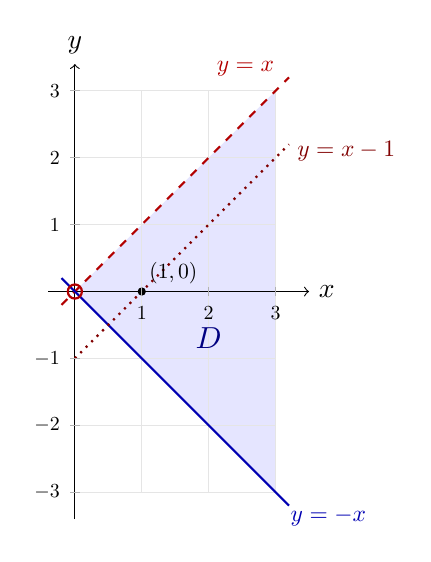
\begin{tikzpicture}[scale=0.85]
  % Shaded domain: triangle (0,0)-(3,-3)-(3,3)
  \fill[blue!10] (0,0) -- (3,-3) -- (3,3) -- cycle;
  % Light grid
  \draw[gray!20, thin] (0,-3) grid[step=1] (3,3);
  % Axes
  \draw[->] (-0.4,0) -- (3.5,0) node[right] {$x$};
  \draw[->] (0,-3.4) -- (0,3.4) node[above] {$y$};
  % y = x (dashed red — EXCLUIDA: x-y=0)
  \draw[thick, dashed, red!70!black] (-0.2,-0.2) -- (3.2,3.2);
  \node[above left, red!70!black, scale=0.85] at (3.1,3.1) {$y=x$};
  % y = -x (solid blue — INCLUIDA: x+y=0)
  \draw[thick, blue!70!black] (-0.2,0.2) -- (3.2,-3.2);
  \node[below right, blue!70!black, scale=0.85] at (3.1,-3.1) {$y=-x$};
  % y = x-1 (dotted — EXCLUIDA dentro del dominio)
  \draw[thick, dotted, red!50!black] (0,-1) -- (3.2,2.2);
  \node[right, red!50!black, scale=0.85] at (3.2,2.1) {$y=x-1$};
  % Open circle at origin (no pertenece al dominio)
  \draw[red!70!black, thick] (0,0) circle (3pt);
  % Point (1,0): y=x-1 intersects x-axis
  \filldraw[black] (1,0) circle (1.5pt)
    node[above right, scale=0.78] {$(1,0)$};
  % Domain label
  \node[blue!50!black, scale=1.1] at (2.0,-0.7) {$D$};
  % Tick marks
  \foreach \x in {1,2,3} {
    \draw[gray!60] (\x,0.07) -- (\x,-0.07);
    \node[below, scale=0.72] at (\x,-0.12) {$\x$};
  }
  \foreach \y in {-3,-2,-1,1,2,3} {
    \draw[gray!60] (0.07,\y) -- (-0.07,\y);
    \node[left, scale=0.72] at (-0.12,\y) {$\y$};
  }
\end{tikzpicture}
\caption{Dominio de $f(x,y)=\frac{\sqrt{x+y}}{\ln(x-y)}$ (región azul): acotado por $y=-x$ (incluida, trazo sólido) y $y=x$ (excluida, rayado), con la recta $y=x-1$ excluida del interior (punteada). El origen no pertenece al dominio.}
\label{fig:dominio_log_raiz}
\end{figure}

\[
\boxed{D = \{(x,y) : x+y \geq 0,\; x-y > 0,\; x-y \neq 1\}}.
\]
\end{myproof}
\end{example}

\begin{prob}
Determine el dominio de la función $f(x,y)=\sqrt{-5x^2-5y^2+25}$. Haga una representación gráfica de este dominio en el plano.
\begin{myproof}
Sea $f(x,y)=\sqrt{-5x^2-5y^2+25}.$ El dominio de la función está dado por los valores de $(x,y)$ que satisfacen la desigualdad $-5x^2-5y^2+25\geq 0.$ Desarrollando esta desigualdad se tiene que:
\begin{align*}
-5x^2-5y^2+25\geq 0 \Leftrightarrow -(5x^2+5y^2)+25\geq 0 \Leftrightarrow 5x^2+5y^2\leq 25.
\end{align*}
Lo cual indica que el dominio de la función son los puntos que están sobre la frontera y el interior de la elipse $5x^2+5y^2=25.$
La gráfica de este dominio se presenta a continuación como la parte rayada dentro de la elipse:
\begin{figure}[H]
\centering
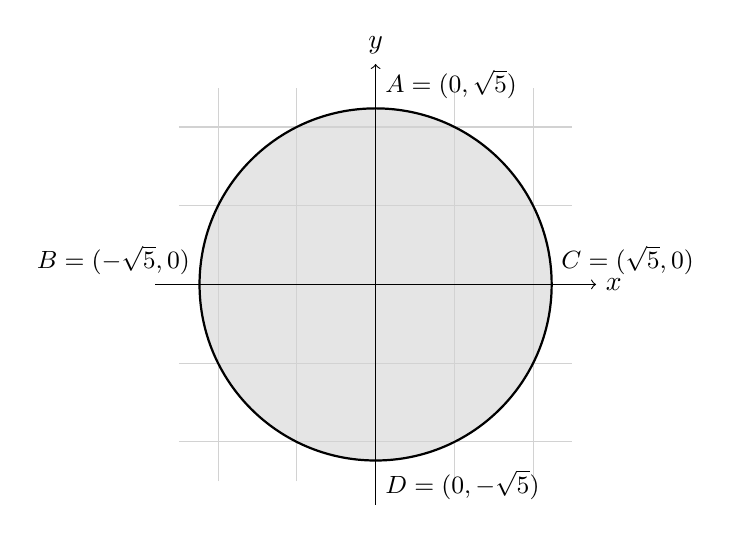
\begin{tikzpicture}[scale=1.0]
  \fill[gray!20] (0,0) circle (2.236);
  \draw[thin,gray!35] (-2.5,-2.5) grid (2.5,2.5);
  \draw[->] (-2.8,0) -- (2.8,0) node[right] {$x$};
  \draw[->] (0,-2.8) -- (0,2.8) node[above] {$y$};
  \draw[thick] (0,0) circle (2.236);
  \node[above right,font=\small] at (2.236,0) {$C=(\sqrt{5},0)$};
  \node[above left,font=\small] at (-2.236,0) {$B=(-\sqrt{5},0)$};
  \node[above right,font=\small] at (0,2.236) {$A=(0,\sqrt{5})$};
  \node[below right,font=\small] at (0,-2.236) {$D=(0,-\sqrt{5})$};
\end{tikzpicture}
\caption{Dominio de $f(x,y)=\sqrt{-5x^2-5y^2+25}$: disco $x^2+y^2\leq 5$}
\label{fig:dom_circulo_5x2y2}
\end{figure}
\end{myproof}
\end{prob}

\begin{prob}
Determine el dominio de la función $f(x,y)=\sqrt{-4x^2-y^2+8}$. Haga una representación gráfica de este dominio en el plano.
\begin{myproof}
Sea $f(x,y)=\sqrt{-4x^2-y^2+8}.$ El dominio de la función está dado por los valores de $(x,y)$ que satisfacen la desigualdad $-4x^2-y^2+8\geq 0.$ Desarrollando esta desigualdad se tiene que:
\begin{align*}
-4x^2-y^2+8\geq 0 \Leftrightarrow -(4x^2+y^2)+8\geq 0 \Leftrightarrow 4x^2+y^2\leq 8.
\end{align*}
Lo cual indica que el dominio de la función son los puntos que están sobre la frontera y el interior de la elipse $4x^2+y^2=8.$
La gráfica de este dominio se presenta a continuación como la parte rayada dentro de la elipse:
\begin{figure}[H]
\centering
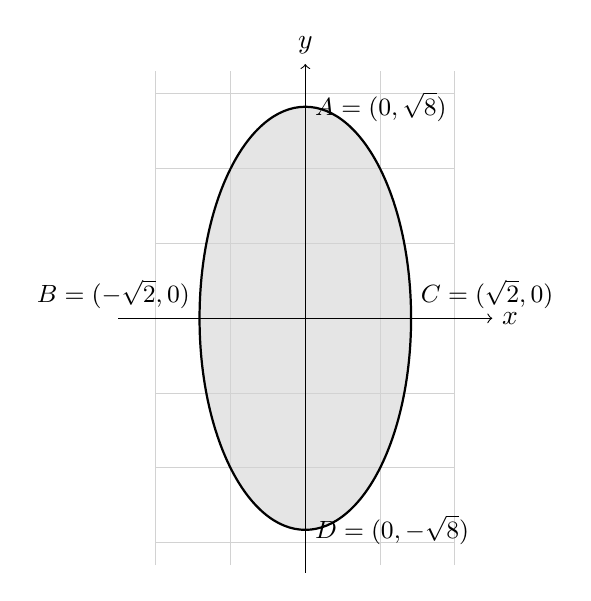
\begin{tikzpicture}[scale=0.95]
  \fill[gray!20] (0,0) ellipse (1.414 and 2.828);
  \draw[thin,gray!35] (-2,-3.3) grid (2,3.3);
  \draw[->] (-2.5,0) -- (2.5,0) node[right] {$x$};
  \draw[->] (0,-3.4) -- (0,3.4) node[above] {$y$};
  \draw[thick] (0,0) ellipse (1.414 and 2.828);
  \node[above right,font=\small] at (1.414,0) {$C=(\sqrt{2},0)$};
  \node[above left,font=\small] at (-1.414,0) {$B=(-\sqrt{2},0)$};
  \node[right,font=\small] at (0,2.828) {$A=(0,\sqrt{8})$};
  \node[right,font=\small] at (0,-2.828) {$D=(0,-\sqrt{8})$};
\end{tikzpicture}
\caption{Dominio de $f(x,y)=\sqrt{-4x^2-y^2+8}$: elipse $4x^2+y^2\leq 8$}
\label{fig:dom_elipse_4x2y2}
\end{figure}
\end{myproof}
\end{prob}

\begin{prob}
Determine el dominio de la función $f(x,y)=\sqrt{-x^2-3y^2+2}$. Haga una representación gráfica de este dominio en el plano.
\begin{myproof}
Sea $f(x,y)=\sqrt{-x^2-3y^2+2}.$ El dominio de la función está dado por los valores de $(x,y)$ que satisfacen la desigualdad $-x^2-3y^2+2\geq 0.$ Desarrollando esta desigualdad se tiene que:
\begin{align*}
-x^2-3y^2+2\geq 0 \Leftrightarrow -(x^2+3y^2)+2\geq 0 \Leftrightarrow x^2+3y^2\leq 2.
\end{align*}
Lo cual indica que el dominio de la función son los puntos que están sobre la frontera y el interior de la elipse $x^2+3y^2=2.$
La gráfica de este dominio se presenta a continuación como la parte rayada dentro de la elipse:
\begin{figure}[H]
\centering
\begin{tikzpicture}[scale=1.3]
  \fill[gray!20] (0,0) ellipse (1.414 and 0.816);
  \draw[thin,gray!35] (-1.8,-1.1) grid (1.8,1.1);
  \draw[->] (-1.9,0) -- (1.9,0) node[right] {$x$};
  \draw[->] (0,-1.2) -- (0,1.2) node[above] {$y$};
  \draw[thick] (0,0) ellipse (1.414 and 0.816);
  \node[above right,font=\small] at (1.414,0) {$C=(\sqrt{2},0)$};
  \node[above left,font=\small] at (-1.414,0) {$A=(-\sqrt{2},0)$};
  \node[above right,font=\small] at (0,0.816) {$B=\!\left(0,\sqrt{\tfrac{2}{3}}\right)$};
  \node[below right,font=\small] at (0,-0.816) {$D=\!\left(0,-\sqrt{\tfrac{2}{3}}\right)$};
\end{tikzpicture}
\caption{Dominio de $f(x,y)=\sqrt{-x^2-3y^2+2}$: elipse $x^2+3y^2\leq 2$}
\label{fig:dom_elipse_x2_3y2}
\end{figure}
\end{myproof}
\end{prob}

% [Original: líneas 310-331 | solución completa | PSTRICKS - pendiente convertir a tikz | 2 variante(s) de parámetro (se descartaron 1)]
\begin{prob}
Determine el dominio de la función $f(x,y)=\sqrt{-3x^2-3y^2+9}$. Haga una representación gráfica de este dominio en el plano.
\begin{myproof}
Sea $f(x,y)=\sqrt{-3x^2-3y^2+9}.$ El dominio de la función está dado por los valores de $(x,y)$ que satisfacen la desigualdad $-3x^2-3y^2+9\geq 0.$ Desarrollando esta desigualdad se tiene que:
\begin{align*}
-3x^2-3y^2+9\geq 0 \Leftrightarrow -(3x^2+3y^2)+9\geq 0 \Leftrightarrow 3x^2+3y^2\leq 9.
\end{align*}
Lo cual indica que el dominio de la función son los puntos que están sobre la frontera y el interior de la elipse $3x^2+3y^2=9.$
La gráfica de este dominio se presenta a continuación como la parte rayada dentro de la elipse:
\begin{figure}[H]
\centering
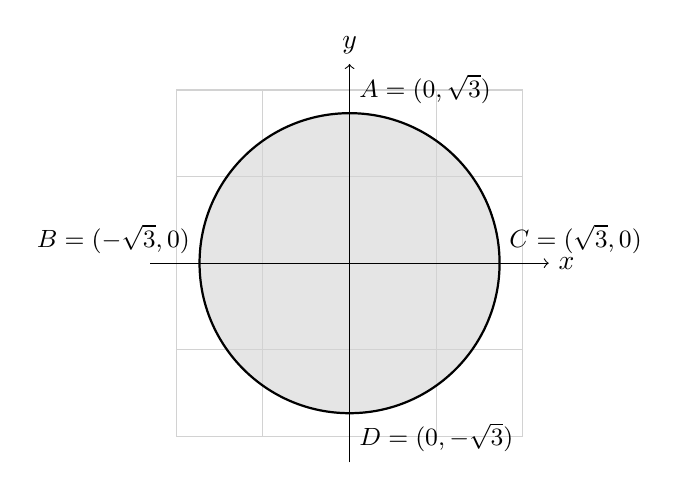
\begin{tikzpicture}[scale=1.1]
  \fill[gray!20] (0,0) circle (1.732);
  \draw[thin,gray!35] (-2,-2) grid (2,2);
  \draw[->] (-2.3,0) -- (2.3,0) node[right] {$x$};
  \draw[->] (0,-2.3) -- (0,2.3) node[above] {$y$};
  \draw[thick] (0,0) circle (1.732);
  \node[above right,font=\small] at (1.732,0) {$C=(\sqrt{3},0)$};
  \node[above left,font=\small] at (-1.732,0) {$B=(-\sqrt{3},0)$};
  \node[above right,font=\small] at (0,1.732) {$A=(0,\sqrt{3})$};
  \node[below right,font=\small] at (0,-1.732) {$D=(0,-\sqrt{3})$};
\end{tikzpicture}
\caption{Dominio de $f(x,y)=\sqrt{-3x^2-3y^2+9}$: disco $x^2+y^2\leq 3$}
\label{fig:dom_circulo_3x2y2}
\end{figure}
\end{myproof}
\end{prob}

\begin{rem}[Dominio en funciones de tres variables]
Para funciones de tres variables, el dominio es una región en el
espacio; las condiciones son análogas, y la descripción se da en
términos de conjuntos de ternas $(x,y,z)$.
\end{rem}

\subsection{Gráfica de una función de dos variables}

La \textbf{gráfica} de una función de dos variables $f(x,y)$ es el
conjunto de puntos $(x,y,z) \in \mathbb{R}^3$ tales que
$z = f(x,y)$. Esta gráfica es, en general, una \textbf{superficie} en
el espacio tridimensional.

Por ejemplo, la función $f(x,y) = x^2 + y^2$ tiene como gráfica un
paraboloide circular: al variar $x$ e $y$, el valor de $z$ aumenta
formando una superficie curva que se abre hacia arriba.

\begin{rem}[Superficies notables]
Muchas superficies que aparecen en aplicaciones son \textbf{superficies
cuadráticas}, definidas por ecuaciones polinómicas de segundo grado en
$x$, $y$ y $z$:
\[
Ax^2 + By^2 + Cz^2 + Dxy + Exz + Fyz + Gx + Hy + Iz + J = 0.
\]
Entre ellas se incluyen el elipsoide, el paraboloide, el hiperboloide y
el cono. La identificación y el trazado de estas superficies se
presenta en la subsección siguiente.
\end{rem}

\subsection{Superficies cuádricas}
\label{sec:superficies-cuadricas}

Una \textbf{superficie cuádrica} es la gráfica en $\mathbb{R}^3$ de una
ecuación polinómica de segundo grado en $x$, $y$, $z$. Toda superficie
cuádrica no degenerada se reduce, mediante traslaciones y rotaciones, a
una de las cinco formas canónicas siguientes. Para identificar una:
(1)~determinar el dominio y rango de $z$; (2)~calcular las trazas con
$z=k$, $y=0$ y $x=0$; (3)~comparar con las formas canónicas; (4)~esbozar.

% ---------- 1. Paraboloide elíptico ----------
\medskip
\noindent\textbf{1.\ Paraboloide elíptico:}
$\dfrac{x^2}{a^2}+\dfrac{y^2}{b^2}=\dfrac{z}{c}$, $c>0$.
Trazas $z=k>0$ son elipses; trazas en planos verticales son parábolas
abriéndose en la dirección de $+z$; vértice en el origen.

\begin{figure}[H]
\centering
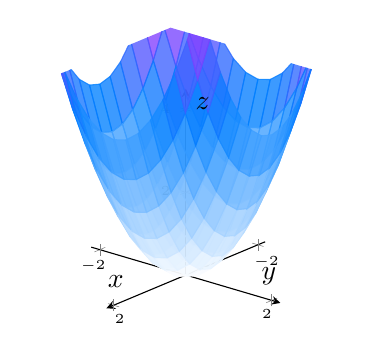
\begin{tikzpicture}
\begin{axis}[axis lines=center, xlabel=$x$, ylabel=$y$, zlabel=$z$,
             xmin=-2.2,xmax=2.2,ymin=-2.2,ymax=2.2,zmin=0,zmax=4.5,
             view={130}{25}, ticklabel style={font=\tiny},
             width=6cm, height=5.5cm]
  \addplot3[surf, shader=flat corner, samples=15, domain=-2:2,
            colormap/cool, opacity=0.78] {x^2+y^2};
\end{axis}
\end{tikzpicture}
\caption{Paraboloide elíptico $z=x^2+y^2$.}
\label{fig:paraboloide_eliptico}
\end{figure}

\begin{example}[Paraboloide elíptico]
Identificar y esbozar la superficie $z = x^2 + 4y^2$.
\begin{myproof}
\textbf{Paso 1.} $D=\mathbb{R}^2$, $z\ge 0$.

\textbf{Paso 2. Trazas.}
$z=k>0$: $x^2+4y^2=k$ (elipses);
$y=0$: $z=x^2$ (parábola $\cup$);
$x=0$: $z=4y^2$ (parábola $\cup$).

\textbf{Paso 3.} Trazas horizontales elípticas y verticales parabólicas
abriéndose hacia arriba: \emph{paraboloide elíptico} con vértice en el
origen.

\textbf{Paso 4.}
\[\boxed{z=x^2+4y^2:\;\text{paraboloide elíptico, vértice }(0,0,0).}\]
\end{myproof}
\end{example}

% ---------- 2. Paraboloide hiperbólico ----------
\medskip
\noindent\textbf{2.\ Paraboloide hiperbólico (silla de montar):}
$z=\dfrac{x^2}{a^2}-\dfrac{y^2}{b^2}$.
Trazas $z=k$ son hipérbolas; la traza $y=0$ es parábola $\cup$ y la
traza $x=0$ es parábola $\cap$; punto de silla en el origen.

\begin{figure}[H]
\centering
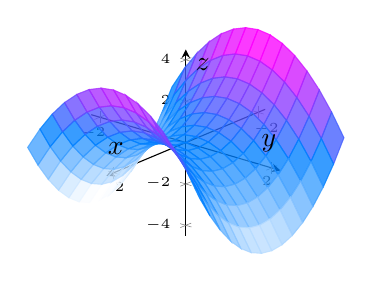
\begin{tikzpicture}
\begin{axis}[axis lines=center, xlabel=$x$, ylabel=$y$, zlabel=$z$,
             xmin=-2.2,xmax=2.2,ymin=-2.2,ymax=2.2,zmin=-4.5,zmax=4.5,
             view={130}{25}, ticklabel style={font=\tiny},
             width=6cm, height=5.5cm]
  \addplot3[surf, shader=flat corner, samples=15, domain=-2:2,
            colormap/cool, opacity=0.78] {x^2-y^2};
\end{axis}
\end{tikzpicture}
\caption{Paraboloide hiperbólico $z=x^2-y^2$ (silla de montar).}
\label{fig:paraboloide_hiperbolico}
\end{figure}

\begin{example}[Paraboloide hiperbólico]
Identificar y esbozar la superficie $z = x^2 - y^2$.
\begin{myproof}
\textbf{Paso 1.} $D=\mathbb{R}^2$, $z\in\mathbb{R}$.

\textbf{Paso 2. Trazas.}
$z=k$: $x^2-y^2=k$ (hipérbolas);
$y=0$: $z=x^2$ (parábola $\cup$);
$x=0$: $z=-y^2$ (parábola $\cap$).

\textbf{Paso 3.} Curvatura opuesta en las dos direcciones principales:
\emph{paraboloide hiperbólico}. El origen es un punto de silla (mínimo
en la dirección $x$, máximo en la dirección $y$).

\textbf{Paso 4.}
\[\boxed{z=x^2-y^2:\;\text{paraboloide hiperbólico, punto de silla }(0,0,0).}\]
\end{myproof}
\end{example}

% ---------- 3. Cono elíptico ----------
\medskip
\noindent\textbf{3.\ Cono elíptico:}
$\dfrac{x^2}{a^2}+\dfrac{y^2}{b^2}=\dfrac{z^2}{c^2}$.
Trazas $z=k\ne0$ son elipses; trazas en planos verticales son pares de
rectas; vértice (punto de pinzamiento) en el origen.

\begin{figure}[H]
\centering
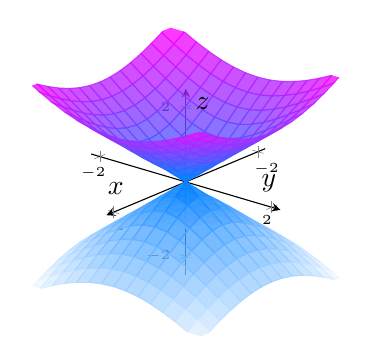
\begin{tikzpicture}
\begin{axis}[axis lines=center, xlabel=$x$, ylabel=$y$, zlabel=$z$,
             xmin=-2.2,xmax=2.2,ymin=-2.2,ymax=2.2,zmin=-2.5,zmax=2.5,
             view={130}{25}, ticklabel style={font=\tiny},
             width=6cm, height=5.5cm]
  \addplot3[surf, shader=flat corner, samples=15, domain=-2:2,
            colormap/cool, opacity=0.78] {sqrt(x^2+y^2)};
  \addplot3[surf, shader=flat corner, samples=15, domain=-2:2,
            colormap/cool, opacity=0.78] {-sqrt(x^2+y^2)};
\end{axis}
\end{tikzpicture}
\caption{Cono circular $z^2=x^2+y^2$, con ambas napas.}
\label{fig:cono_circular}
\end{figure}

\begin{example}[Cono circular]
Identificar y esbozar la superficie $z^2 = x^2 + y^2$.
\begin{myproof}
\textbf{Paso 1.} $z=\pm\sqrt{x^2+y^2}$; $D=\mathbb{R}^2$.

\textbf{Paso 2. Trazas.}
$z=k\ne0$: $x^2+y^2=k^2$ (circunferencia de radio $|k|$);
$y=0$: $z=\pm x$ (dos rectas);
$x=0$: $z=\pm y$ (dos rectas).

\textbf{Paso 3.} Trazas horizontales circulares que se anulan en el
vértice: \emph{cono circular} con dos napas simétricas respecto a $z=0$.

\textbf{Paso 4.}
\[\boxed{z^2=x^2+y^2:\;\text{cono circular, vértice }(0,0,0).}\]
\end{myproof}
\end{example}

% ---------- 4. Hiperboloide de una hoja ----------
\medskip
\noindent\textbf{4.\ Hiperboloide de una hoja:}
$\dfrac{x^2}{a^2}+\dfrac{y^2}{b^2}-\dfrac{z^2}{c^2}=1$.
Trazas $z=k$ son elipses de radio creciente con $|k|$; trazas
verticales son hipérbolas; cintura (radio mínimo) en $z=0$.

\begin{figure}[H]
\centering
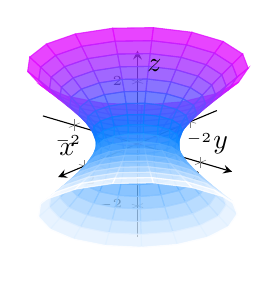
\begin{tikzpicture}
\begin{axis}[axis lines=center, xlabel=$x$, ylabel=$y$, zlabel=$z$,
             xmin=-3,xmax=3,ymin=-3,ymax=3,zmin=-3,zmax=3,
             view={130}{25}, ticklabel style={font=\tiny},
             width=6cm, height=5.5cm]
  \addplot3[surf, shader=flat corner, samples=18,
            colormap/cool, opacity=0.78,
            variable=\u, variable y=\v,
            domain=0:360, y domain=-2.5:2.5,
            trig format plots=deg]
           ({sqrt(1+\v*\v)*cos(\u)}, {sqrt(1+\v*\v)*sin(\u)}, {\v});
\end{axis}
\end{tikzpicture}
\caption{Hiperboloide de una hoja $x^2+y^2-z^2=1$.}
\label{fig:hiperboloide_una_hoja}
\end{figure}

\begin{example}[Hiperboloide de una hoja]
Identificar y esbozar la superficie $x^2 + y^2 - z^2 = 1$.
\begin{myproof}
\textbf{Paso 1.} $x^2+y^2=1+z^2\ge 1$ para todo $z\in\mathbb{R}$.

\textbf{Paso 2. Trazas.}
$z=k$: $x^2+y^2=1+k^2$ (circunferencia de radio $\sqrt{1+k^2}$, mínimo $1$ en $k=0$);
$y=0$: $x^2-z^2=1$ (hipérbola).

\textbf{Paso 3.} Superficie conectada, secciones horizontales circulares
con radio mínimo $1$ en $z=0$: \emph{hiperboloide de una hoja}.

\textbf{Paso 4.}
\[\boxed{x^2+y^2-z^2=1:\;\text{hiperboloide de una hoja, cintura de radio }1.}\]
\end{myproof}
\end{example}

% ---------- 5. Hiperboloide de dos hojas ----------
\medskip
\noindent\textbf{5.\ Hiperboloide de dos hojas:}
$-\dfrac{x^2}{a^2}-\dfrac{y^2}{b^2}+\dfrac{z^2}{c^2}=1$.
Trazas $z=k$ ($|k|\ge c$) son elipses; la superficie tiene dos
componentes separadas ($z\ge c$ y $z\le -c$).

\begin{figure}[H]
\centering
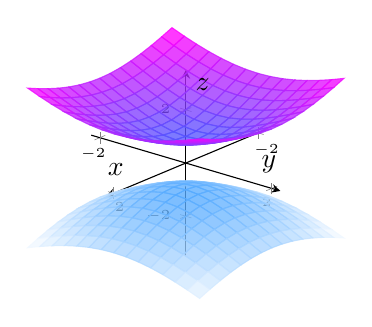
\begin{tikzpicture}
\begin{axis}[axis lines=center, xlabel=$x$, ylabel=$y$, zlabel=$z$,
             xmin=-2.2,xmax=2.2,ymin=-2.2,ymax=2.2,zmin=-3.5,zmax=3.5,
             view={130}{25}, ticklabel style={font=\tiny},
             width=6cm, height=5.5cm]
  \addplot3[surf, shader=flat corner, samples=15, domain=-2:2,
            colormap/cool, opacity=0.78] {sqrt(1+x^2+y^2)};
  \addplot3[surf, shader=flat corner, samples=15, domain=-2:2,
            colormap/cool, opacity=0.78] {-sqrt(1+x^2+y^2)};
\end{axis}
\end{tikzpicture}
\caption{Hiperboloide de dos hojas $z^2-x^2-y^2=1$.}
\label{fig:hiperboloide_dos_hojas}
\end{figure}

\begin{example}[Hiperboloide de dos hojas]
Identificar y esbozar la superficie $z^2 - x^2 - y^2 = 1$.
\begin{myproof}
\textbf{Paso 1.} $z^2=1+x^2+y^2\ge 1$, luego $|z|\ge 1$: dos hojas
disjuntas ($z\ge 1$ y $z\le -1$).

\textbf{Paso 2. Trazas.}
$z=k$ ($|k|\ge1$): $x^2+y^2=k^2-1$ (circunferencias vacías para $|k|<1$);
$y=0$: $z^2-x^2=1$ (hipérbola).

\textbf{Paso 3.} Dos casquetes separados por la condición $|z|\ge 1$:
\emph{hiperboloide de dos hojas}, con puntos más cercanos al origen en
$(0,0,\pm1)$.

\textbf{Paso 4.}
\[\boxed{z^2-x^2-y^2=1:\;\text{hiperboloide de dos hojas, puntos }(0,0,\pm1).}\]
\end{myproof}
\end{example}

\subsection{Curvas y superficies de nivel}

Las \textbf{curvas de nivel} son una herramienta fundamental para
visualizar funciones de dos variables sin necesidad de construir su
gráfica tridimensional. Una curva de nivel está formada por todos los
puntos del dominio donde la función toma un valor constante.

\begin{definition}[Curva de nivel]
Sea $f(x,y)$ una función de dos variables. Para un número real $k$, la
\textbf{curva de nivel} $k$ de $f$ es el conjunto
\[
C_k = \{(x,y) \in \operatorname{Dom}(f) : f(x,y) = k\}.
\]
El conjunto de varias curvas de nivel para distintos valores de $k$ se
denomina \textbf{mapa de contorno}.
\end{definition}

Geométricamente, si $z = f(x,y)$ es una superficie en el espacio, la
intersección de esta superficie con el plano horizontal $z = k$ es una
curva en el espacio. La proyección de dicha curva sobre el plano $xy$
es la curva de nivel correspondiente.

\begin{definition}[Superficie de nivel]
Para una función de tres variables $f(x,y,z)$, una \textbf{superficie
de nivel} es el conjunto de puntos $(x,y,z)$ del dominio que satisfacen
$f(x,y,z) = k$ para un valor fijo de $k$.
\end{definition}

Las superficies de nivel permiten visualizar regiones del espacio donde
la función mantiene un valor constante, facilitando la comprensión de
fenómenos tridimensionales como campos de temperatura, presión o
potencial.

\begin{pasos}[Trazado de curvas de nivel]
Para dibujar las curvas de nivel de $f(x,y)$:
\begin{enumerate}
  \item \textbf{Elegir valores de $k$.} Seleccionar una secuencia de
        valores representativos, por ejemplo, $k = -2, -1, 0, 1, 2$ o
        valores que revelen la forma de la función.
  \item \textbf{Igualar $f(x,y) = k$.} Para cada $k$, escribir la
        ecuación resultante.
  \item \textbf{Identificar la curva.} Reconocer la curva en el plano
        $xy$ (circunferencia, elipse, recta, parábola, etc.).
  \item \textbf{Dibujar.} Representar todas las curvas en el mismo
        sistema de coordenadas, etiquetando cada una con su valor $k$.
\end{enumerate}
\end{pasos}

\begin{figure}[H]
\centering
\begin{minipage}{0.46\textwidth}
\centering
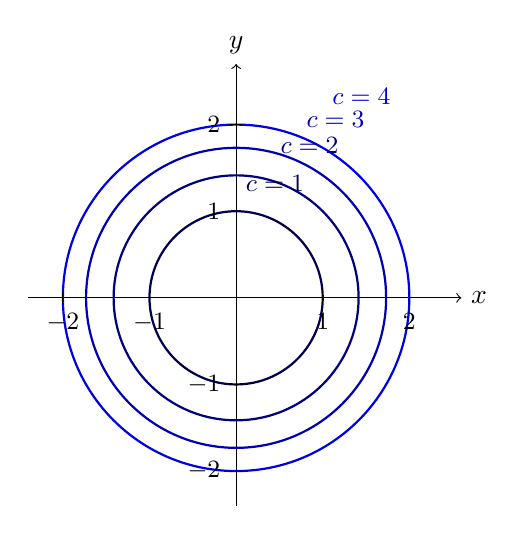
\begin{tikzpicture}[scale=1.1]
    \draw[thin,->] (-2.4,0) -- (2.6,0) node[right] {$x$};
    \draw[thin,->] (0,-2.4) -- (0,2.7) node[above] {$y$};
    \draw[thick, blue!30!black] (0,0) circle (1.0);
    \draw[thick, blue!50!black] (0,0) circle (1.414);
    \draw[thick, blue!70!black] (0,0) circle (1.732);
    \draw[thick, blue!90!black] (0,0) circle (2.0);
    \node[anchor=south west, blue!30!black] at (0.0, 1.12) {\small $c=1$};
    \node[anchor=south west, blue!50!black] at (0.4, 1.55) {\small $c=2$};
    \node[anchor=south west, blue!70!black] at (0.7, 1.85) {\small $c=3$};
    \node[anchor=south west, blue!90!black] at (1.0, 2.12) {\small $c=4$};
    \foreach \x in {-2,-1,1,2}
        \draw[thin] (\x,0.07)--(\x,-0.07) node[below] {\small $\x$};
    \foreach \y in {-2,-1,1,2}
        \draw[thin] (0.07,\y)--(-0.07,\y) node[left] {\small $\y$};
\end{tikzpicture}
\end{minipage}
\hfill
\begin{minipage}{0.50\textwidth}
\centering
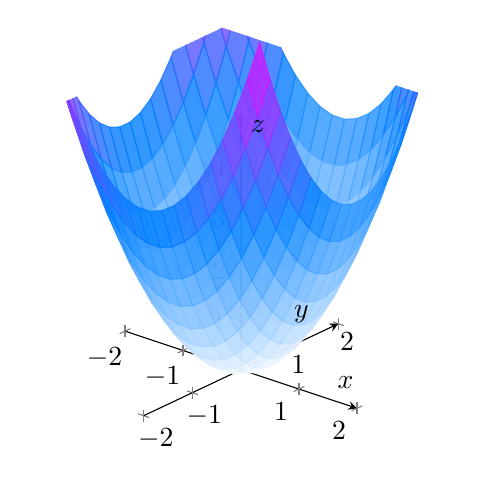
\begin{tikzpicture}
\begin{axis}[
    view={40}{25},
    xlabel={$x$}, ylabel={$y$}, zlabel={$z$},
    axis lines=center,
    tick style={thin},
    zmin=0, zmax=5,
    xtick={-2,-1,1,2}, ytick={-2,-1,1,2}, ztick={1,2,3,4},
    width=7cm, height=7cm,
]
    \addplot3[
        surf, shader=flat corner,
        samples=20, domain=-2:2,
        opacity=0.80, colormap/cool,
    ] {x^2 + y^2};
\end{axis}
\end{tikzpicture}
\end{minipage}
\caption{Paraboloide $z=x^2+y^2$: curvas de nivel $c=1,2,3,4$
         en el plano $xy$ (izquierda) y superficie en $\mathbb{R}^3$ (derecha)}
\label{fig:paraboloide_curvas_nivel}
\end{figure}

\begin{example}[Curvas de nivel de un paraboloide]
Dibujar las curvas de nivel de $f(x,y) = x^2 + y^2$ para
$k = 0, 1, 4, 9$.
\begin{myproof}
\textbf{Paso 1. Elegir valores de $k$.}
Los valores dados son $k = 0, 1, 4, 9$.

\textbf{Paso 2. Igualar $f(x,y) = k$.}
Para cada $k$:
\[
x^2 + y^2 = k.
\]

\textbf{Paso 3. Identificar la curva.}
La ecuación $x^2 + y^2 = k$ representa:
\begin{itemize}
  \item Para $k=0$: el punto $(0,0)$.
  \item Para $k>0$: una circunferencia centrada en el origen con radio
        $\sqrt{k}$.
\end{itemize}

\textbf{Paso 4. Dibujar.}
Las curvas de nivel son circunferencias concéntricas de radios
$0, 1, 2, 3$, correspondientes a $k=0,1,4,9$.

\begin{figure}[H]
\centering
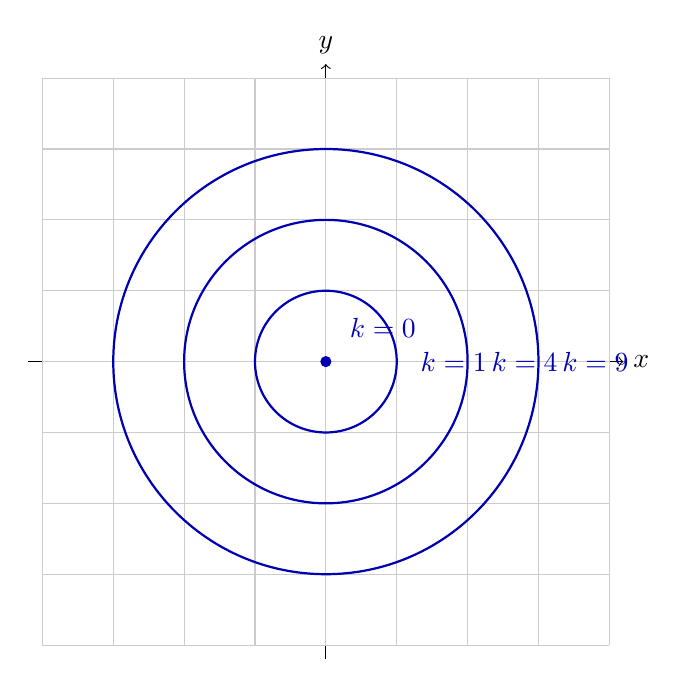
\begin{tikzpicture}[scale=0.9]
  \draw[->] (-4.2,0) -- (4.2,0) node[right] {$x$};
  \draw[->] (0,-4.2) -- (0,4.2) node[above] {$y$};
  \draw[thin, gray!40] (-4,-4) grid (4,4);
  \draw[blue!70!black, thick] (0,0) circle (1);
  \draw[blue!70!black, thick] (0,0) circle (2);
  \draw[blue!70!black, thick] (0,0) circle (3);
  \filldraw[blue!70!black] (0,0) circle (2pt);
  \node[blue!70!black, anchor=west] at (1.2, 0) {$k=1$};
  \node[blue!70!black, anchor=west] at (2.2, 0) {$k=4$};
  \node[blue!70!black, anchor=west] at (3.2, 0) {$k=9$};
  \node[blue!70!black, anchor=south west] at (0.2, 0.2) {$k=0$};
\end{tikzpicture}
\caption{Curvas de nivel de $f(x,y)=x^2+y^2$ para $k=0,1,4,9$}
\label{fig:curvas_nivel_paraboloide}
\end{figure}

\[
\boxed{\text{Las curvas de nivel son circunferencias concéntricas con centro en el origen.}}
\]
\end{myproof}
\end{example}

\begin{rem}[Interpretación en topografía]
En un mapa topográfico, las curvas de nivel unen puntos de igual
altitud. Si $f(x,y)$ representa la altura del terreno en el punto
$(x,y)$, las curvas de nivel son las líneas de contorno del mapa.
\end{rem}

% ---- Ejemplos de superficies de nivel f(x,y,z)=k (F8.27) ----

\begin{example}[Superficies de nivel: familia de esferas]
Describir las superficies de nivel de $f(x,y,z) = x^2+y^2+z^2$ para
$k=1$, $k=4$ y $k=9$.
\begin{myproof}
\textbf{Paso 1. Dominio.} $D=\mathbb{R}^3$, $f\ge 0$. Solo $k\ge 0$
produce superficies no vacías.

\textbf{Paso 2. Ecuación de nivel.} Para cada $k>0$:
\[
x^2+y^2+z^2 = k
\quad\Longrightarrow\quad
\text{esfera centrada en el origen con radio }\sqrt{k}.
\]
Para $k=0$: solo el punto origen. Para $k<0$: conjunto vacío.

\textbf{Paso 3. Familia.} Al aumentar $k$ las esferas se expanden
concéntricamente. Los valores $k=1,4,9$ dan radios $1, 2, 3$.

\begin{figure}[H]
\centering
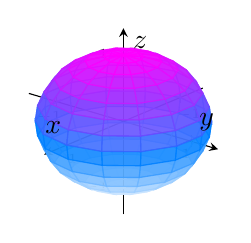
\begin{tikzpicture}
\begin{axis}[axis lines=center, xlabel=$x$, ylabel=$y$, zlabel=$z$,
             xmin=-1.4,xmax=1.4,ymin=-1.4,ymax=1.4,zmin=-1.4,zmax=1.4,
             view={130}{25}, ticklabel style={font=\tiny},
             width=6cm, height=5.5cm]
  \addplot3[surf, shader=flat corner, samples=15,
            colormap/cool, opacity=0.78,
            variable=\u, variable y=\v,
            domain=0:360, y domain=0:180,
            trig format plots=deg]
           ({cos(\u)*sin(\v)}, {sin(\u)*sin(\v)}, {cos(\v)});
\end{axis}
\end{tikzpicture}
\caption{Superficie de nivel $k=1$: esfera unitaria $x^2+y^2+z^2=1$.}
\label{fig:nivel_esfera}
\end{figure}

\textbf{Paso 4.}
\[\boxed{f(x,y,z)=x^2+y^2+z^2=k:\;
\text{esferas de radio }\sqrt{k}\text{ centradas en el origen.}}\]
\end{myproof}
\end{example}

\begin{example}[Superficie de nivel: elipsoide]
Describir la superficie de nivel $k=1$ de
$\displaystyle f(x,y,z)=x^2+\frac{y^2}{4}+\frac{z^2}{9}$.
\begin{myproof}
\textbf{Paso 1. Dominio.} $D=\mathbb{R}^3$, $f\ge 0$.

\textbf{Paso 2. Ecuación de nivel $k=1$.}
\[
x^2+\frac{y^2}{4}+\frac{z^2}{9}=1:
\quad\text{forma estándar de elipsoide con semiejes }a=1,\,b=2,\,c=3.
\]

\textbf{Paso 3. Identificación.} La superficie es compacta y convexa,
contenida en el cubo $[-1,1]\times[-2,2]\times[-3,3]$. Al variar $k$
se obtiene la familia $\tfrac{x^2}{k}+\tfrac{y^2}{4k}+\tfrac{z^2}{9k}=1$
(elipsoides homoteticos).

\begin{figure}[H]
\centering
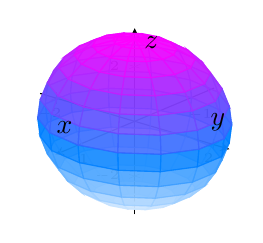
\begin{tikzpicture}
\begin{axis}[axis lines=center, xlabel=$x$, ylabel=$y$, zlabel=$z$,
             xmin=-1.4,xmax=1.4,ymin=-2.4,ymax=2.4,zmin=-3.4,zmax=3.4,
             view={130}{25}, ticklabel style={font=\tiny},
             width=6cm, height=5.5cm]
  \addplot3[surf, shader=flat corner, samples=15,
            colormap/cool, opacity=0.78,
            variable=\u, variable y=\v,
            domain=0:360, y domain=0:180,
            trig format plots=deg]
           ({cos(\u)*sin(\v)}, {2*sin(\u)*sin(\v)}, {3*cos(\v)});
\end{axis}
\end{tikzpicture}
\caption{Superficie de nivel $k=1$: elipsoide con semiejes $a=1$, $b=2$, $c=3$.}
\label{fig:nivel_elipsoide}
\end{figure}

\textbf{Paso 4.}
\[\boxed{k=1:\;\text{elipsoide }x^2+\tfrac{y^2}{4}+\tfrac{z^2}{9}=1,
\;\text{semiejes }1,\,2,\,3.}\]
\end{myproof}
\end{example}

\begin{example}[Superficies de nivel: familia de paraboloides]
Describir las superficies de nivel de $f(x,y,z) = x^2+y^2-z$ para
$k=0$, $k=1$ y $k=-1$.
\begin{myproof}
\textbf{Paso 1. Dominio.} $D=\mathbb{R}^3$, $f\in\mathbb{R}$.

\textbf{Paso 2. Ecuación de nivel.} $x^2+y^2-z=k$ equivale a
\[
z = x^2+y^2-k.
\]
Cada nivel $k$ es un \emph{paraboloide circular} abierto hacia arriba
con vértice en $(0,0,-k)$.

\textbf{Paso 3. Familia.} Al aumentar $k$ el vértice desciende (se
aleja hacia $-z$); al disminuir $k$, asciende. Las superficies son
paraboloides congruentes desplazados verticalmente.

\begin{figure}[H]
\centering
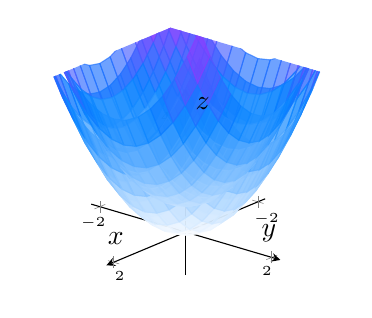
\begin{tikzpicture}
\begin{axis}[axis lines=center, xlabel=$x$, ylabel=$y$, zlabel=$z$,
             xmin=-2.2,xmax=2.2,ymin=-2.2,ymax=2.2,zmin=-1.5,zmax=5,
             view={130}{25}, ticklabel style={font=\tiny},
             width=6cm, height=5.5cm]
  \addplot3[surf, shader=flat corner, samples=15, domain=-2:2,
            colormap/cool, opacity=0.78] {x^2+y^2};
  \addplot3[surf, shader=flat corner, samples=15, domain=-2:2,
            colormap/cool, opacity=0.65] {x^2+y^2+1};
\end{axis}
\end{tikzpicture}
\caption{Familia de paraboloides $z=x^2+y^2-k$: $k=0$ vértice en $z=0$ (abajo) y
         $k=-1$ vértice en $z=1$ (arriba).}
\label{fig:nivel_paraboloides}
\end{figure}

\textbf{Paso 4.}
\[\boxed{f(x,y,z)=x^2+y^2-z=k:\;\text{paraboloide }z=x^2+y^2-k,
\;\text{vértice en }(0,0,-k).}\]
\end{myproof}
\end{example}

\begin{prob}
Tome la función $f(x,y)=\ln\left(1+8x^2+2y^2\right).$
\begin{enumerate}[(a)]
    \item Calcule el dominio de $f(x,y).$ Grafique este dominio.
    \item Construya en el plano las curvas de nivel para los valores $z=0,1,2,4.$
\end{enumerate}
\begin{myproof}
\begin{enumerate}[(a)]
\item Sea $f(x,y)=\ln\left(1+8x^2+2y^2\right).$ El dominio de la función está dado por los valores de $(x,y)$ que satisfacen la desigualdad $1+8x^2+2y^2> 0.$ Desarrollando esta desigualdad se tiene que cualquier punto del plano la satisface, por lo tanto, el dominio de la función es el plano $\mathbb{R}^2.$ Un bosquejo puede ser el siguiente
\begin{figure}[H]
\centering
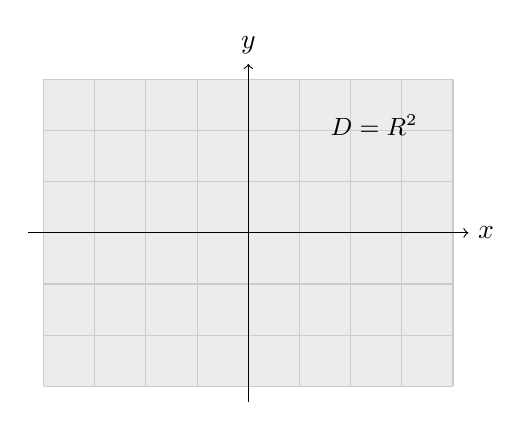
\begin{tikzpicture}[scale=0.65]
  \fill[gray!15] (-4,-3) rectangle (4,3);
  \draw[thin,gray!40] (-4,-3) grid (4,3);
  \draw[->] (-4.3,0) -- (4.3,0) node[right] {$x$};
  \draw[->] (0,-3.3) -- (0,3.3) node[above] {$y$};
  \node[anchor=north east, font=\small] at (3.5,2.5) {$D=\mathbb{R}^2$};
\end{tikzpicture}
\caption{Dominio de $f(x,y)=\ln(1+8x^2+2y^2)$: todo $\mathbb{R}^2$}
\label{fig:dom_ln_8x2_2y2}
\end{figure}
\item Al calcular las curvas de nivel se tiene que:
\begin{itemize}
\item Para $z=0$ la ecuación es $0=\ln\left( 1+8x^2+2y^2 \right).$ Solucionando:
\begin{align*}
0=\ln\left( 1+8x^2+2y^2 \right)&\Rightarrow \mathrm{e}^{0}=\mathrm{e}^{\ln\left( 1+8x^2+2y^2 \right)}\\ &\Rightarrow 1=1+2y^2+8x^2 \Rightarrow 0=2y^2+8x^2\\ &\Rightarrow  x=0\text{ y } y=0.
\end{align*}
 y así la curva de nivel es el punto $(0,0).$
\item Para $z=1$: $(e-1) = 8x^2+2y^2$, elipse con semiejes $a_x=\sqrt{(e-1)/8}\approx 0.463$, $a_y=\sqrt{(e-1)/2}\approx 0.927$.
\item Para $z=2$: $(e^2-1) = 8x^2+2y^2$, elipse con semiejes $a_x\approx 0.894$, $a_y\approx 1.787$.
\item Para $z=4$: $(e^4-1) = 8x^2+2y^2$, elipse con semiejes $a_x\approx 2.589$, $a_y\approx 5.177$.
\end{itemize}
La gráfica de las curvas de nivel se presenta a continuación:
\begin{figure}[H]
\centering
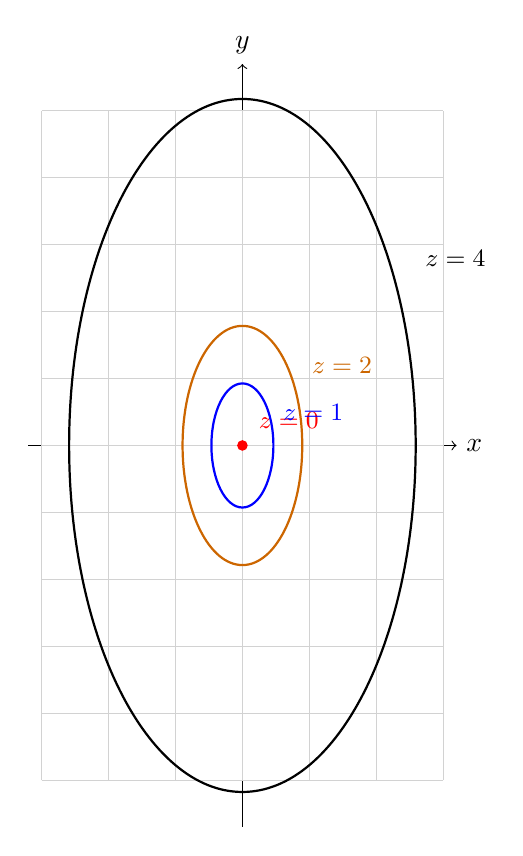
\begin{tikzpicture}[scale=0.85]
  \draw[->] (-3.2,0) -- (3.2,0) node[right] {$x$};
  \draw[->] (0,-5.7) -- (0,5.7) node[above] {$y$};
  \draw[thin,gray!35] (-3,-5) grid (3,5);
  \filldraw[red] (0,0) circle (2pt);
  \node[red,above right,font=\small] at (0.1,0.1) {$z=0$};
  \draw[blue,thick] (0,0) ellipse (0.463 and 0.927);
  \node[blue,right,font=\small] at (0.463,0.5) {$z=1$};
  \draw[orange!80!black,thick] (0,0) ellipse (0.894 and 1.787);
  \node[orange!80!black,right,font=\small] at (0.894,1.2) {$z=2$};
  \draw[thick] (0,0) ellipse (2.589 and 5.177);
  \node[anchor=west, font=\small] at (2.589,2.8) {$z=4$};
\end{tikzpicture}
\caption{Curvas de nivel de $f(x,y)=\ln(1+8x^2+2y^2)$ para $z=0,1,2,4$}
\label{fig:nivel_ln_8x2_2y2}
\end{figure}
\end{enumerate}
\end{myproof}
\end{prob}

\begin{prob}
Tome la función $f(x,y)=\ln\left(1+4x^2+y^2\right).$
\begin{enumerate}[(a)]
    \item Calcule el dominio de $f(x,y).$ Grafique este dominio.
    \item Construya en el plano las curvas de nivel para los valores $z=0,1,2,5.$
\end{enumerate}
\begin{myproof}
\begin{enumerate}[(a)]
\item Sea $f(x,y)=\ln\left(1+4x^2+y^2\right).$ El dominio de la función está dado por los valores de $(x,y)$ que satisfacen la desigualdad $1+4x^2+y^2> 0.$ Desarrollando esta desigualdad se tiene que cualquier punto del plano la satisface, por lo tanto, el dominio de la función es el plano $\mathbb{R}^2.$ Un bosquejo puede ser el siguiente
\begin{figure}[H]
\centering
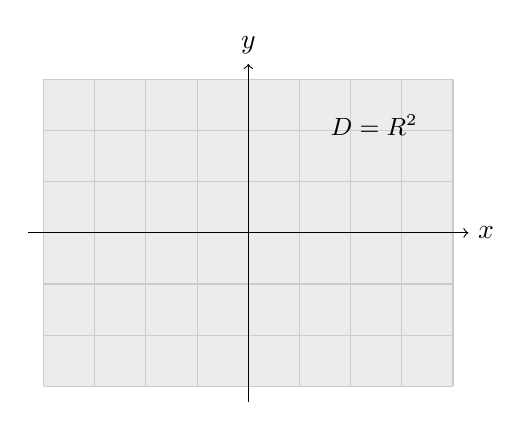
\begin{tikzpicture}[scale=0.65]
  \fill[gray!15] (-4,-3) rectangle (4,3);
  \draw[thin,gray!40] (-4,-3) grid (4,3);
  \draw[->] (-4.3,0) -- (4.3,0) node[right] {$x$};
  \draw[->] (0,-3.3) -- (0,3.3) node[above] {$y$};
  \node[anchor=north east, font=\small] at (3.5,2.5) {$D=\mathbb{R}^2$};
\end{tikzpicture}
\caption{Dominio de $f(x,y)=\ln(1+4x^2+y^2)$: todo $\mathbb{R}^2$}
\label{fig:dom_ln_4x2_y2}
\end{figure}
\item Al calcular las curvas de nivel se tiene que:
\begin{itemize}
\item Para $z=0$: el punto $(0,0)$.
\item Para $z=1$: $(e-1) = 4x^2+y^2$, elipse con semiejes $a_x\approx 0.655$, $a_y\approx 1.310$.
\item Para $z=2$: $(e^2-1) = 4x^2+y^2$, elipse con semiejes $a_x\approx 1.264$, $a_y\approx 2.528$.
\item Para $z=5$: $(e^5-1) = 4x^2+y^2$, elipse con semiejes $a_x\approx 6.071$, $a_y\approx 12.141$.
\end{itemize}
La gráfica de las curvas de nivel se presenta a continuación:
\begin{figure}[H]
\centering
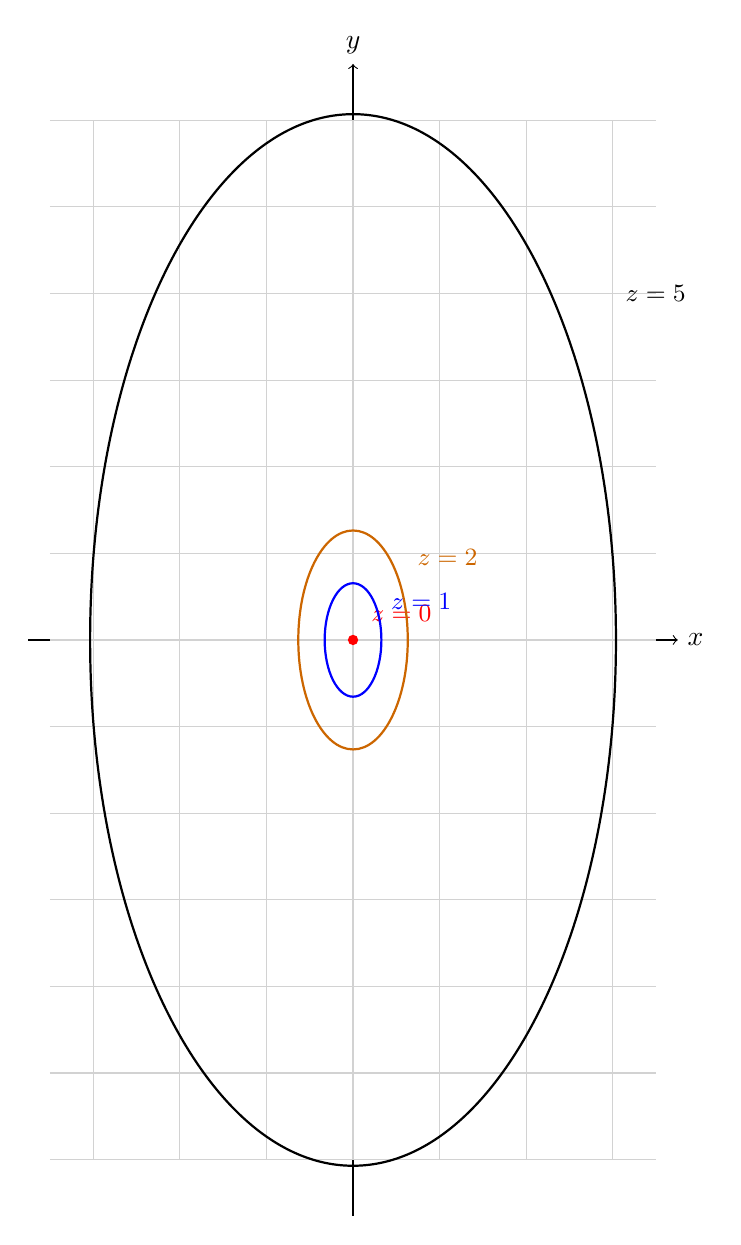
\begin{tikzpicture}[scale=0.55]
  \draw[->] (-7.5,0) -- (7.5,0) node[right] {$x$};
  \draw[->] (0,-13.3) -- (0,13.3) node[above] {$y$};
  \draw[thin,gray!35] (-7,-12) grid[step=2] (7,12);
  \filldraw[red] (0,0) circle (3pt);
  \node[red,above right,font=\small] at (0.2,0.2) {$z=0$};
  \draw[blue,thick] (0,0) ellipse (0.655 and 1.310);
  \node[blue,right,font=\small] at (0.655,0.9) {$z=1$};
  \draw[orange!80!black,thick] (0,0) ellipse (1.264 and 2.528);
  \node[orange!80!black,right,font=\small] at (1.264,1.9) {$z=2$};
  \draw[thick] (0,0) ellipse (6.071 and 12.141);
  \node[anchor=west, font=\small] at (6.071,8) {$z=5$};
\end{tikzpicture}
\caption{Curvas de nivel de $f(x,y)=\ln(1+4x^2+y^2)$ para $z=0,1,2,5$}
\label{fig:nivel_ln_4x2_y2}
\end{figure}
\end{enumerate}
\end{myproof}
\end{prob}

\section{Problemas propuestos}
\label{sec:problems-L1.1}


\begin{prob}
Determinar si las siguientes funciones vectoriales son continuas en $t=0$:
\begin{enumerate}[a)]
  \item $\mathbf{r}(t) = \left\langle \frac{\sen t}{t},\; \cos t \right\rangle$.
  \item $\mathbf{r}(t) = \left\langle t^2,\; \frac{1}{t},\; e^t \right\rangle$.
  \item $\mathbf{r}(t) = \left\langle t^3,\; \frac{\sen t}{t},\; \frac{t^2-1}{t-1} \right\rangle$
        (definir $\mathbf{r}(0)=\langle 0,1,2\rangle$).
\end{enumerate}
\end{prob}



\begin{prob}
Calcular las siguientes integrales definidas e indefinidas:
\begin{enumerate}[a)]
  \item $\displaystyle \int \langle t^2,\; 3t,\; \sen t \rangle\,dt$.
  \item $\displaystyle \int_0^1 \langle e^t,\; t^3,\; \cos(\pi t) \rangle\,dt$.
  \item $\displaystyle \int_0^{\pi/2} \langle \sen t \cos t,\; \cos^2 t,\; t \rangle\,dt$.
\end{enumerate}
\end{prob}



\begin{prob}
Encontrar la función longitud de arco $s(t)$ para $\mathbf{r}(t) = \langle t,\; t^2 \rangle$
desde $t=0$. Reparametrizar la curva en términos de $s$ (expresar el
resultado como integral si no es posible hallar una forma elemental).
\end{prob}

\begin{prob}
Determinar el dominio de las siguientes funciones de dos variables:
\begin{enumerate}[a)]
  \item $f(x,y) = \sqrt{x+y}$.
  \item $f(x,y) = \ln(xy)$.
  \item $f(x,y) = \dfrac{1}{\sqrt{x^2 + y^2 - 1}}$.
  \item $f(x,y) = \dfrac{\ln(x-y+1)}{\sqrt{x^2+y^2-4}}$.
  \item $f(x,y) = \arcsin(x+y)$.
\end{enumerate}
\end{prob}

\begin{prob}
Describir y esbozar el dominio de:
\begin{enumerate}[a)]
  \item $f(x,y) = \sqrt{4 - x^2 - y^2}$.
  \item $f(x,y) = \ln(1 - x^2 - y^2)$.
  \item $f(x,y) = \dfrac{1}{x^2 + y^2 - 1}$.
  \item $f(x,y) = \sqrt{x^2 + y^2 - 4} + \ln(9 - x^2 - y^2)$.
\end{enumerate}
\end{prob}

\begin{prob}
Dibujar las curvas de nivel para los valores de $k$ indicados:
\begin{enumerate}[a)]
  \item $f(x,y) = x + y$,\quad $k = -2, -1, 0, 1, 2$.
  \item $f(x,y) = x^2 - y^2$,\quad $k = -4, -1, 0, 1, 4$.
  \item $f(x,y) = xy$,\quad $k = -2, -1, 0, 1, 2$.
  \item $f(x,y) = \sqrt{x^2 + y^2}$,\quad $k = 1, 2, 3$.
\end{enumerate}
\end{prob}

\begin{prob}
Describir las curvas de nivel de $f(x,y) = x^2 + 4y^2$. ¿Qué relación
tienen con la gráfica de $f$?
\end{prob}

\begin{prob}
Identificar y esbozar la gráfica de las siguientes funciones:
\begin{enumerate}[a)]
  \item $z = \sqrt{x^2 + y^2}$ (cono).
  \item $z = 4 - x^2 - y^2$ (paraboloide).
  \item $z = \sqrt{9 - x^2 - y^2}$ (semiesfera).
  \item $z = x^2 + y^2$ (paraboloide circular).
\end{enumerate}
\end{prob}

\begin{prob}
Para la función $f(x,y) = x^2 + y^2$:
\begin{enumerate}[a)]
  \item Encontrar la curva de nivel para $k=1$.
  \item ¿Qué representa geométricamente la curva de nivel?
  \item ¿Cuál es la ecuación de la superficie $z = f(x,y)$?
  \item Describir la intersección de la superficie con el plano $z=1$.
\end{enumerate}
\end{prob}

\begin{prob}
Para la función $f(x,y,z) = x^2 + y^2 + z^2$:
\begin{enumerate}[a)]
  \item Describir las superficies de nivel para $k>0$.
  \item ¿Qué ocurre para $k=0$?
  \item ¿Qué representa geométricamente la superficie de nivel $k=1$?
\end{enumerate}
\end{prob}


\begin{prob}
Considere las siguientes funciones de varias variables. Para cada una determine su dominio $D$, grafique en el plano $XY$ o en el espacio $XYZ$ el dominio de la función.
\begin{multicols}{2}
\begin{enumerate}[(a)]
    \item $f(x,y)=\sqrt{2x-y}.$
    \item $f(x,y)=\ln\left(9-x^2-9y^2\right).$
    \item $f(x,y)=\sqrt{y}+\sqrt{25-x^2-y^2}.$
    \item $f(x,y)=\dfrac{\sqrt{x^2-y}}{1-x^2}.$
    \item $f(x,y)=\arcsin\left( x^2+y^2-2 \right).$
    \item $f(x,y,z)=\ln\left(9-x^2-9y^2+z\right).$
    \item $f(x,y,z)=\sqrt{1-x^2-y^2-z^2}+\ln(xyz).$
    \item $f(x,y,z)=\sqrt{x+y+z}+\sqrt{x}+\sqrt{y}+\sqrt{z}.$
    \item $f(x,y,z)=z\ln(xy).$
    \item $f(x,y,z)=\sqrt{144-16x^2-9y^2-144z^2}.$
    \item $f(x,y,z)=e^{\sqrt{x^2-y^2-z^2}}.$
\end{enumerate}
\end{multicols}
\end{prob}


\begin{prob}
Haga un bosquejo de la gráfica de las siguientes funciones de dos variables.
\begin{multicols}{2}
\begin{enumerate}[(a)]
    \item  $f(x,y)=10.$
    \item  $f(x,y)=6-x-2y.$
    \item  $f(x,y)=y^2-x^2+1.$
    \item $f(x,y)=x^2-\frac{y^2}{4}.$
    \item $f(x,y)=x^2+4y^2.$
    \item $f(x,y)=\sqrt{1-25x^2+y^2}.$
    \item $f(x,y)=\sqrt{1+x^2+y^2}.$
\end{enumerate}
\end{multicols}
\end{prob}


\begin{prob}
Para cada una de las siguientes funciones construya las curvas de nivel o las superficies de nivel, según corresponda, para cada uno de los valores indicados:
\begin{enumerate}[(a)]
    \item $z=6-2x-3y,$ $z=0,2,4,6,8,10.$
    \item $f(x,y)=\ln(x-y),$ $z=0,\pm \frac{1}{2},\pm 1, \pm \frac{3}{2},\pm 2.$ 
    \item $f(x,y)=\dfrac{x^2+1}{x^2+y^2},$ $z=1,2,4,6.$
    \item $f(x,y)=\sqrt{9-x^2-y^2},$ $z=0,1,2,3.$
    \item $f(x,y)=x^2-y^2,$ $z=-4,-3,-2,-1,0,1,2,3.$
    \item $f(x,y,z)=100x^2+16y^2+25z^2,$ $w=0,1,2,3,4.$
    \item $f(x,y,z)=x^2-y^2+z^2.$ $w=0,1,2,3.$
    \item $f(x,y,z)=x^2+y^2+z^2-4x-6y+15z.$ $w=0,1,2,3.$
    \item $f(x,y,z)=x^2-y^2-z^2.$ $w=0,1,2,3.$
\end{enumerate}
\end{prob}


\begin{prob}
Grafique la curvas de nivel de la función $f(x,y)=\sqrt{25-5x^2-3y^2}$ para los valores de $z=0,2,5.$
\end{prob}


\begin{prob}
Grafique la curvas de nivel de la función $f(x,y)=\sqrt{36-x^2-5y^2}$ para los valores de $z=0,3,6.$
\end{prob}


